\documentclass{article}
\usepackage{graphicx}
\graphicspath{ {./report_img/} } % graphics path
\usepackage{fancyhdr}
\usepackage{listings}
\setlength{\parindent}{0pt}
\usepackage{float}
\usepackage[letterpaper,margin=1in]{geometry}
\renewcommand{\baselinestretch}{1.2}    % line spacing
\usepackage{amsmath}
\usepackage{amssymb} % for \mathbb -- set of integers
%\usepackage[bf,large]{caption}
\usepackage{caption}
\usepackage{subcaption} % for subfigure environment
\usepackage{steinmetz}  % for \phase
\usepackage{mathrsfs}   % for \mathscr -- Laplace transform operator
\usepackage{mathtools}  % for \floor{}
\usepackage{sectsty}
\usepackage[usenames,dvipsnames]{color}
\definecolor{lightgray}{gray}{0.5}
% This is the color used for MATLAB comments below
\definecolor{MyDarkGreen}{rgb}{0.0,0.4,0.0}
\lstloadlanguages{Matlab}%
\lstset{language=bash,                        % Use MATLAB
        frame=single,                           % Single frame around code
        basicstyle=\small\ttfamily,             % Use small true type font
        %keywordstyle=[1]\color{Blue}\bf,        % MATLAB functions bold and blue
        %keywordstyle=[2]\color{Purple},         % MATLAB function arguments purple
        %keywordstyle=[3]\color{Blue}\underbar,  % User functions underlined and blue
        identifierstyle=,                       % Nothing special about identifiers
                                                % Comments small dark green courier
        commentstyle=\usefont{T1}{pcr}{m}{sl}\color{MyDarkGreen}\small,
        stringstyle=\color{Purple},             % Strings are purple
        showstringspaces=false,                 % Don't put marks in string spaces
        tabsize=2,                              % 5 spaces per tab
        %
        morecomment=[l][\color{Blue}]{...},     % Line continuation (...) like blue comment
        numbers=left,                           % Line numbers on left
        firstnumber=0,                          % Line numbers start with line 1
        numberstyle=\tiny\color{Blue},          % Line numbers are blue
        stepnumber=1,                           % Line numbers go in steps of 5
        breaklines=true
        }
\pagestyle{fancy}
%\thispagestyle{plain}

\def\class{ECE 408}
\def\fp{Final Project}

\partfont{\centering}

\lhead{ Sun, Xue, Miao, \class, \fp}

\begin{document}

\title{\fp}
\date{} % disable date to include in the title
\author{
\begin{tabular}{ccc}
    Alvin Sun & Yuqi Xue & Yan Miao \tabularnewline
    yixiaos3 & yuqixue2 & yanmiao2
\end{tabular}
}
%\maketitle

\begin{titlepage} % Suppresses displaying the page number on the title page and the subsequent page counts as page 1
	\newcommand{\HRule}{\rule{\linewidth}{0.5mm}} % Defines a new command for horizontal lines, change thickness here

	\center % Centre everything on the page

	%------------------------------------------------
	%	Headings
	%------------------------------------------------

	\textsc{\LARGE University of Illinois at Urbana Champaign}\\[1.5cm] % Main heading such as the name of your university/college

	\textsc{\Large Applied Parallel Programming}\\[0.5cm] % Major heading such as course name

	\large Team: wandering-gpu \\[0.5cm] % Minor heading such as course title

	%------------------------------------------------
	%	Title
	%------------------------------------------------

	\HRule\\[0.4cm]

	{\huge\bfseries Final Project}\\[0.4cm] % Title of your document

	\HRule\\[1.5cm]

	%------------------------------------------------
	%	Author(s)
	%------------------------------------------------

	\begin{minipage}{0.4\textwidth}
		\begin{flushleft}
			\large
			\textit{Author}\\
			Alvin Sun \\ % Your name
            Yuqi Xue  \\
            Yan Miao
		\end{flushleft}
	\end{minipage}
	~
	\begin{minipage}{0.4\textwidth}
		\begin{flushright}
			\large
			\textit{Net ID}\\
			yixiaos3 \\ % net id
            yuqixue2 \\
            yanmiao2
		\end{flushright}
	\end{minipage}

	% If you don't want a supervisor, uncomment the two lines below and comment the code above
	%{\large\textit{Author}}\\
	%John \textsc{Smith} % Your name

	%------------------------------------------------
	%	Date
	%------------------------------------------------

	\vfill\vfill\vfill % Position the date 3/4 down the remaining page

	{\large\today} % Date, change the \today to a set date if you want to be precise

	%------------------------------------------------
	%	Logo
	%------------------------------------------------

	%\vfill\vfill
	%\includegraphics[width=0.2\textwidth]{placeholder.jpg}\\[1cm] % Include a department/university logo - this will require the graphicx package

	%----------------------------------------------------------------------------------------

	\vfill % Push the date up 1/4 of the remaining page

\end{titlepage}

% deprecated
% \part*{Credentials}
% \setcounter{section}{0}
%
% \begin{tabular}{ll}
%     \textbf{Team Name}: & wandering-gpu \tabularnewline
%     \textbf{School Affiliation}: & UIUC \tabularnewline
%     \tabularnewline
% \end{tabular} \\
% \begin{tabular}{ll}
%     \textbf{Name}: & Alvin Sun \tabularnewline
%     \textbf{NetID}: & yixiaos3 \tabularnewline
%     \textbf{RaiID}: & 5c78c49784318364bab96ed4 \tabularnewline
%     \tabularnewline
%     \textbf{Name}: & Yuqi Xue \tabularnewline
%     \textbf{NetID}: & yuqixue2 \tabularnewline
%     \textbf{RaiID}: & 5c78c49f84318364bab96ee2 \tabularnewline
%     \tabularnewline
%     \textbf{Name}: & Yan Miao \tabularnewline
%     \textbf{NetID}: & yanmiao2 \tabularnewline
%     \textbf{RaiID}: & 5c78c48d84318364bab96ec2
% \end{tabular}

\part*{Milestone 1}
\setcounter{section}{0}

\section{Kernel Statistics}
\begin{tabular}{ccccccl}
 Time(\%) & Time & Calls & Avg & Min &   Max  &  Name \tabularnewline
  40.10\% &  16.788ms &  20 & 839.42us & 1.1200us & 16.155ms & [CUDA memcpy HtoD] \tabularnewline
  20.18\% & 8.4497ms  &  1 &  8.4497ms & 8.4497ms & 8.4497ms & void cudnn::detail::implicit\_convolve\_sgemm \tabularnewline
  11.81\% & 4.9434ms  &  1 &  4.9434ms & 4.9434ms & 4.9434ms & volta\_cgemm\_64x32\_tn \tabularnewline
   7.05\% & 2.9497ms  &  2 &  1.4748ms & 25.568us & 2.9241ms & void op\_generic\_tensor\_kernel \tabularnewline
   5.69\% & 2.3830ms  &  1 &  2.3830ms & 2.3830ms & 2.3830ms & void fft2d\_c2r\_32x32 \tabularnewline
   5.59\% & 2.3404ms  &  1 &  2.3404ms & 2.3404ms & 2.3404ms & volta\_sgemm\_128x128\_tn \tabularnewline
   4.55\% & 1.9059ms  &  1 &  1.9059ms & 1.9059ms & 1.9059ms & void cudnn::detail::pooling\_fw\_4d\_kernel \tabularnewline
   4.18\% & 1.7480ms  &  1 &  1.7480ms & 1.7480ms & 1.7480ms & void fft2d\_r2c\_32x32
\end{tabular}

\section{CUDA API Statistics}
\begin{tabular}{ccccccl}
Time(\%)   &   Time   &  Calls   &    Avg   &    Min    &   Max  &  Name \tabularnewline
41.94\% & 2.94373s    &    22 & 133.81ms & 13.721us & 1.52482s & cudaStreamCreateWithFlags \tabularnewline
 34.43\% & 2.41664s    &    24 & 100.69ms & 97.853us & 2.41057s & cudaMemGetInfo \tabularnewline
 20.93\% & 1.46898s    &    19 & 77.315ms &    817ns & 393.98ms & cudaFree \tabularnewline
\end{tabular}

\section{Differences Between Kernels \& API Calls} % DONE
% Report: Include an explanation of the difference between kernels and API calls.
A CUDA kernel is an extended C function that, when called, are executed multiple times in parallel by different CUDA threads on the GPU.
The CUDA APIs are programming interfaces that allow the programmer to use the CUDA device, i.e. the GPU.
Kernel functions are written by the programmer and are meant to execute specific (mostly computation-intensive) tasks on the GPU,
while API calls are provided by the CUDA library and are to manage the CUDA runtime environment and mostly prepare for the execution of kernels.
While kernels are always executed by CUDA cores, CUDA APIs do not necessarily involve the execution of CUDA cores.

\section{MXNet CPU Execution}
\begin{lstlisting}[language=bash]
Loading fashion-mnist data... done
Loading model... done
New Inference
EvalMetric: {'accuracy': 0.8236}
\end{lstlisting}

\textbf{Run Time.} 5.06s

\pagebreak
\section{MXNet GPU Execution}
\begin{lstlisting}[language=bash]
Loading fashion-mnist data... done
Loading model... done
New Inference
EvalMetric: {'accuracy': 0.8236}
\end{lstlisting}

\textbf{Run Time:} 4.40s

\part*{Milestone 2}
\setcounter{section}{0}

% \section{CPU Execution Time}
\begin{table}[H]
    \centering
    \begin{minipage}{.32\linewidth}
        \begin{tabular}{c|c}
            Full CPU Time & 11.32s \\ \hline
            First Layer Time & 2.405296s \\ \hline
            Second Layer Time & 7.342860s
        \end{tabular}
        \caption*{10000 images}
    \end{minipage}
    ~
    \begin{minipage}{.32\linewidth}
        \begin{tabular}{c|c}
            Full CPU Time & 0.250576s \\ \hline
            First Layer Time & 0.756567s \\ \hline
            Second Layer Time & 2.03s
        \end{tabular}
        \caption*{1000 images}
    \end{minipage}
    ~
    \begin{minipage}{.32\linewidth}
        \begin{tabular}{c|c}
            Full CPU Time & 1.08s \\ \hline
            First Layer Time & 0.035050s \\ \hline
            Second Layer Time & 0.075312s
        \end{tabular}
        \caption*{100 images}
    \end{minipage}
    \caption{CPU Run Time Statistics}
\end{table}

\part*{Milestone 3}
\setcounter{section}{0}

\section{Execution Summary}

\begin{table}[H]
    \centering
    \begin{minipage}{.32\linewidth}
        \begin{tabular}{c|c}
            Accuracy & 0.8397 \\ \hline
            First Layer Time & 9.252ms \\ \hline
            Second Layer Time & 19.331ms
        \end{tabular}
        \caption*{10000 images}
    \end{minipage}
    ~
    \begin{minipage}{.32\linewidth}
        \begin{tabular}{c|c}
            Accuracy & 0.852 \\ \hline
            First Layer Time & 0.677ms \\ \hline
            Second Layer Time & 1.968ms
        \end{tabular}
        \caption*{1000 images}
    \end{minipage}
    ~
    \begin{minipage}{.32\linewidth}
        \begin{tabular}{c|c}
            Accuracy & 0.84 \\ \hline
            First Layer Time & 0.121ms \\ \hline
            Second Layer Time & 0.248ms
        \end{tabular}
        \caption*{100 images}
    \end{minipage}
    \caption{GPU Run Time Statistics}
\end{table}

\section{Execution Timeline}

\begin{figure}[H]
    \centering
    \begin{subfigure}[b]{\linewidth}
        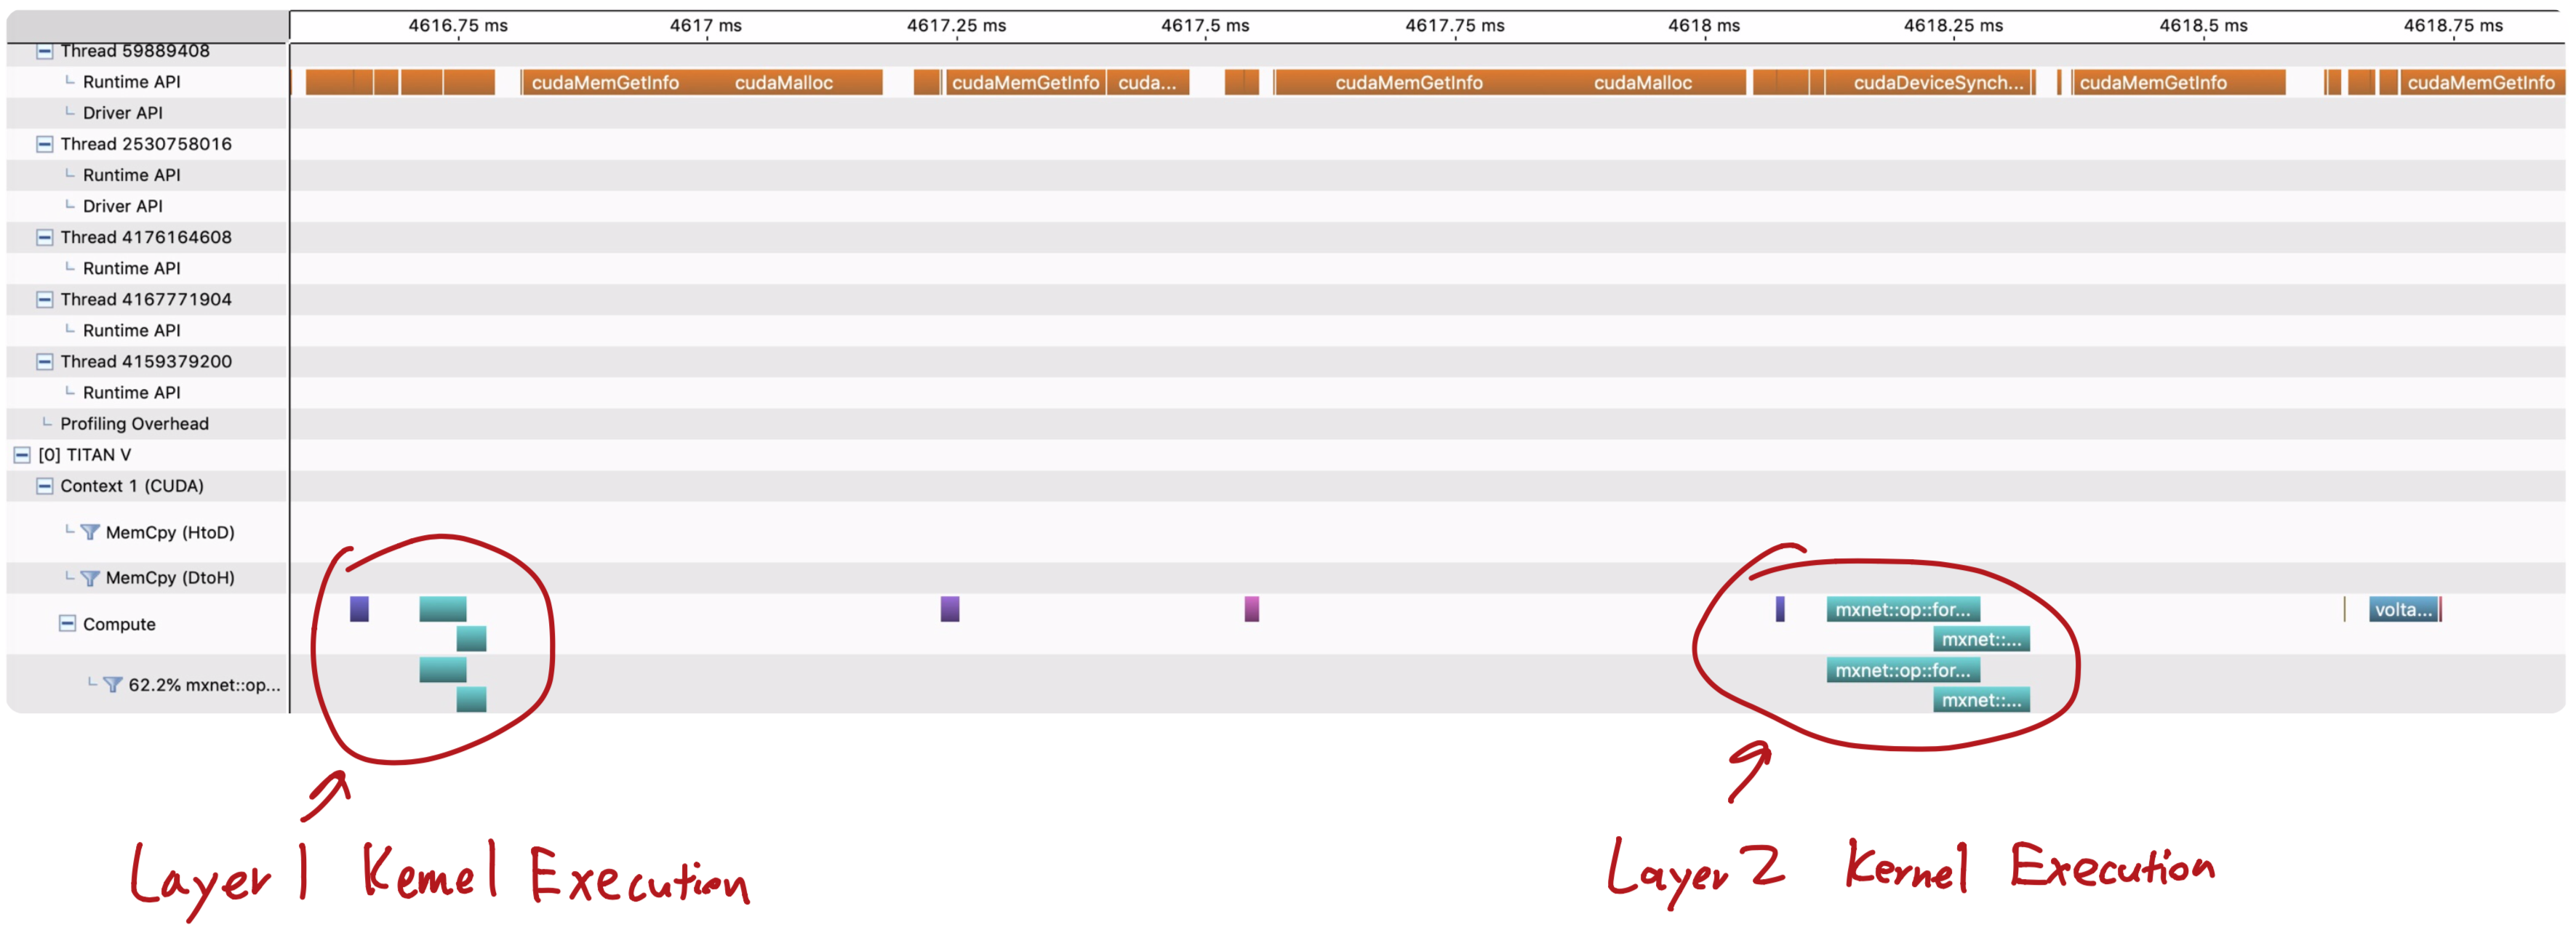
\includegraphics[width=\linewidth]{nvvp100an}
        \caption{Dataset Size 100}
    \end{subfigure}
    \begin{subfigure}[b]{\linewidth}
        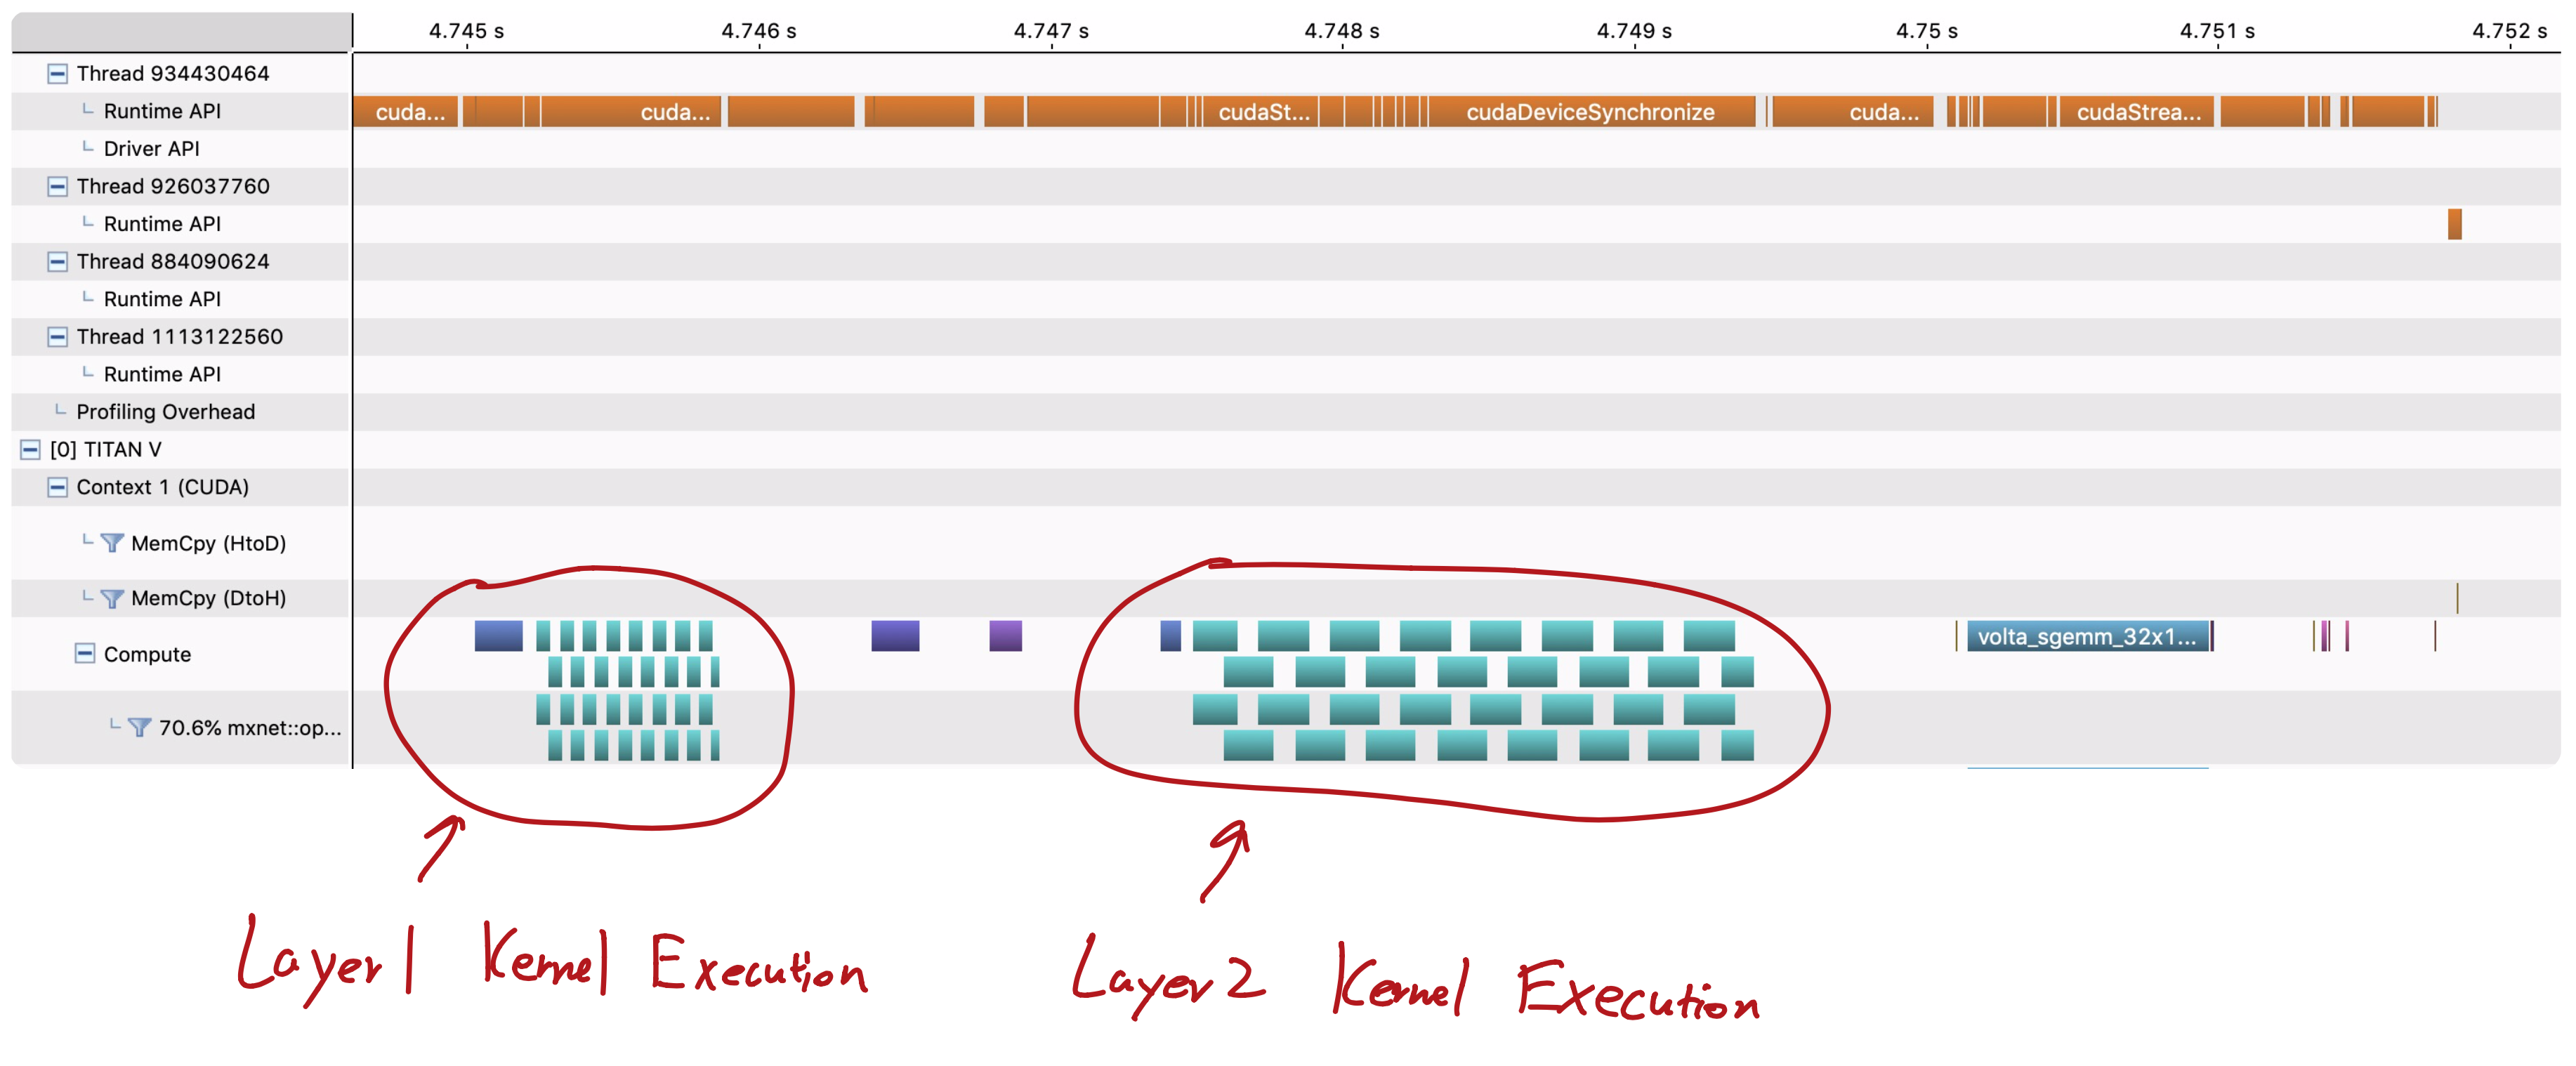
\includegraphics[width=\linewidth]{nvvp1000an}
        \caption{Dataset Size 1000}
    \end{subfigure}
    \begin{subfigure}[b]{\linewidth}
        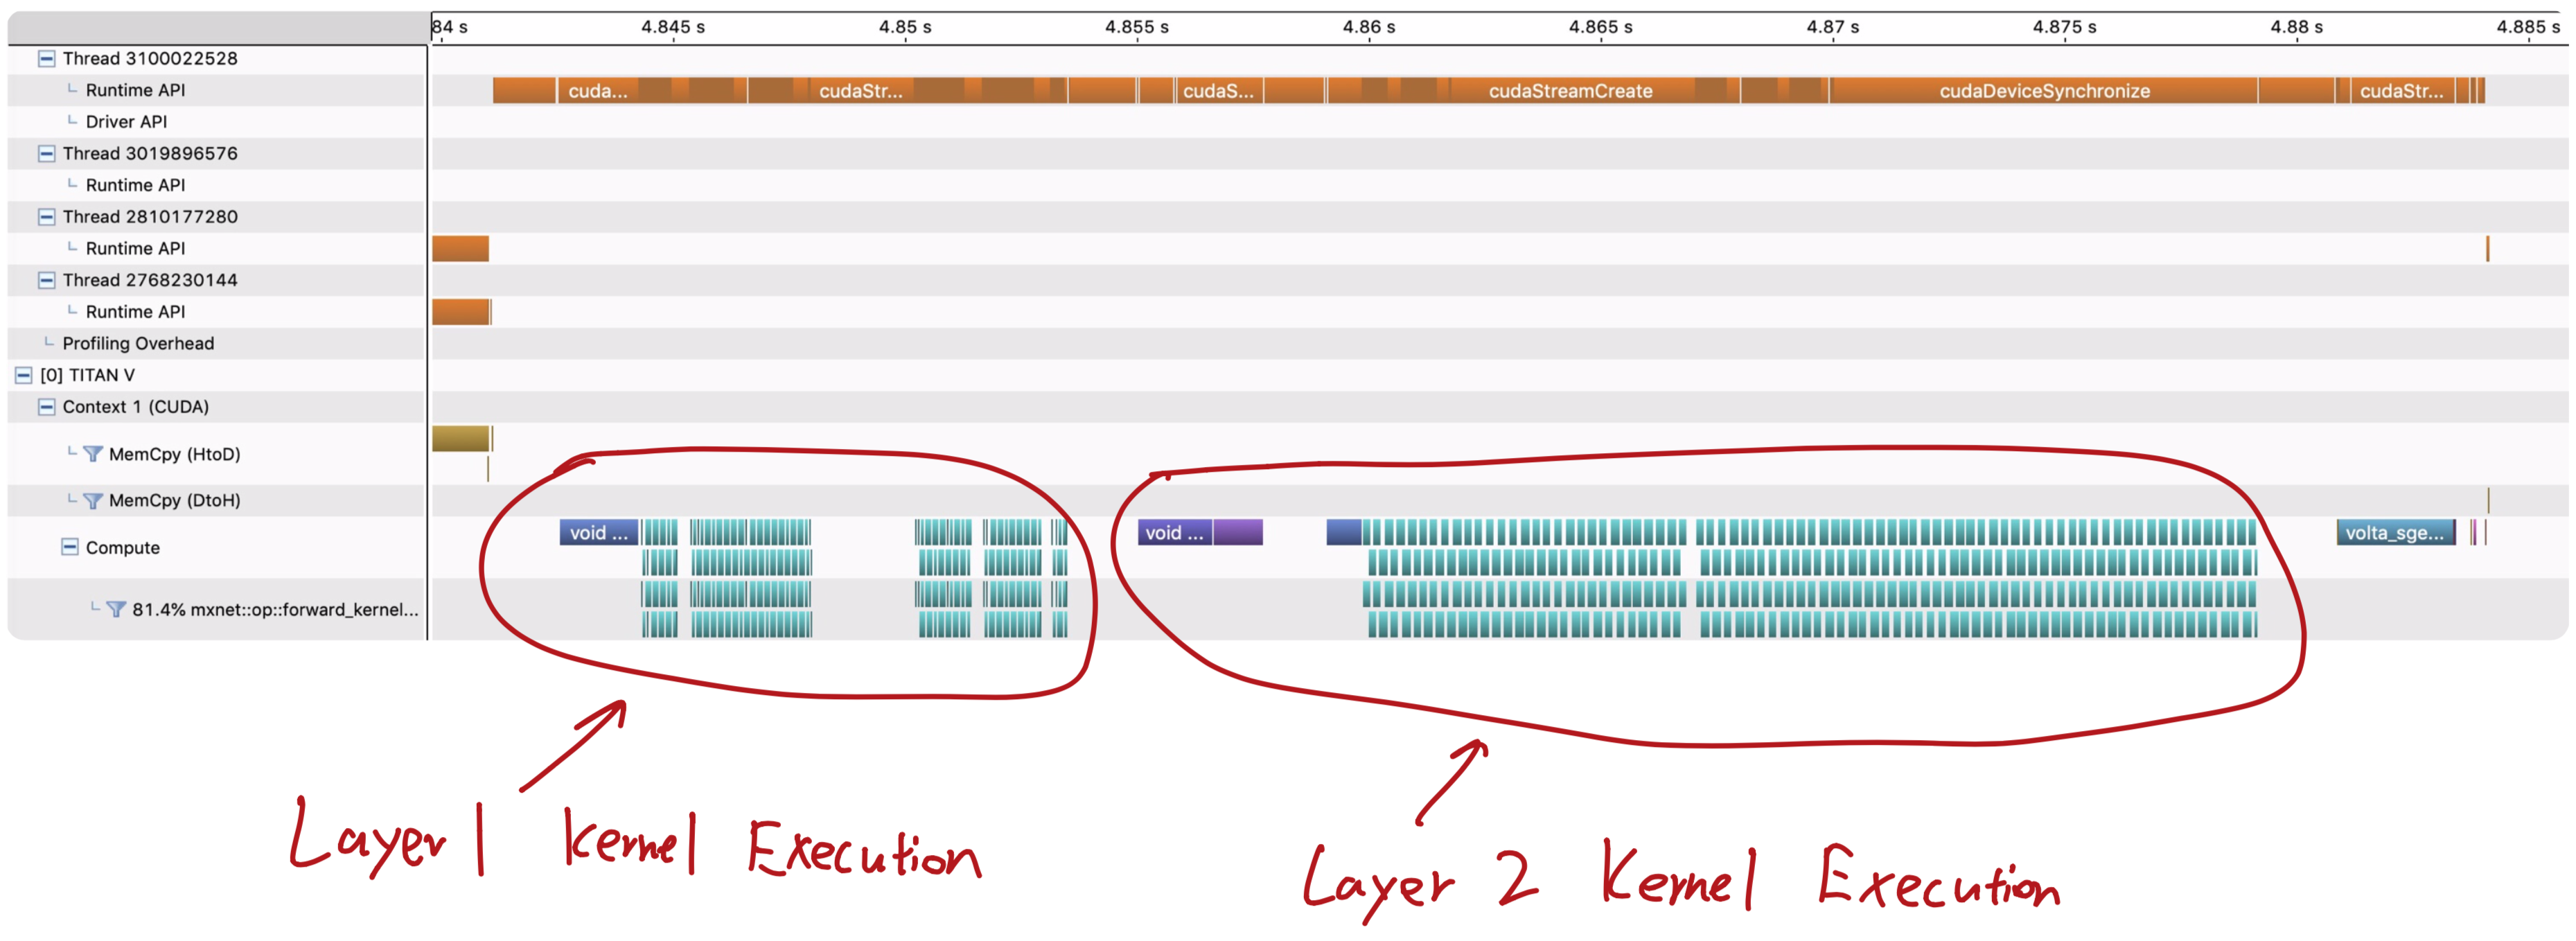
\includegraphics[width=\linewidth]{nvvp10000an}
        \caption{Datset Size 10000}
    \end{subfigure}
    \caption{Kernel Execution Timelines generated by NVVP.}
\end{figure}

\part*{Milestone 4}
\setcounter{section}{0}

\section{Execution Summary}
Upon Milestone 4, we have implemented three optimizations to our kernel function, including having different
implementations and tuning for different layers, using shared memory convolution, and putting convolution
kernels in constant memory. The overall execution (on server) involving all three optimizations yields the following
results.

\begin{table}[H]
    \centering
    \begin{minipage}{.32\linewidth}
        \begin{tabular}{c|c}
            Accuracy & 0.8397 \\ \hline
            First Layer Time & 3.560ms \\ \hline
            Second Layer Time & 12.878ms
        \end{tabular}
        \caption*{10000 images}
    \end{minipage}
    ~
    \begin{minipage}{.32\linewidth}
        \begin{tabular}{c|c}
            Accuracy & 0.852 \\ \hline
            First Layer Time & 0.366ms \\ \hline
            Second Layer Time & 1.180ms
        \end{tabular}
        \caption*{1000 images}
    \end{minipage}
    ~
    \begin{minipage}{.32\linewidth}
        \begin{tabular}{c|c}
            Accuracy & 0.84 \\ \hline
            First Layer Time & 0.074ms \\ \hline
            Second Layer Time & 0.149ms
        \end{tabular}
        \caption*{100 images}
    \end{minipage}
    \caption{Run time statistics after applying all three optimizations.}
\end{table}

We will discuss each optimization in the following section.

\section{Optimizations}

\paragraph{Note}
As a preliminary note, we would like to mention that, in order to avoid unexpected server fluctuations and speedup our development,
we have setup a local development environment using an NVIDIA GeForce RTX 2080 running CUDA 10.0. Our discussions below will be based on
execution results and statistics generated in our local environment. Despite this, we have ensured that our optimizations work as
intended on the server. Also, for simplicity, we will only benchmark data size 10000.

\subsection{Seperate Kernel Implementations for Different Layers}
As far as we observe, the original kernel function, although general enough to be used for both layers, has a function signiture
\begin{verbatim}
__global__ void forward_kernel(float *y, const float *x, const float *k,
        const int B, const int M, const int C, const int H, const int W, const int K)
\end{verbatim}
that is too long and many of the parameters are unnecessary as we already know them for each layer. Hence, one optimization involves
implementing two different kernel functions for these two different layers. In other words, this optimization is barely finding and hardcoding
the best possible parameters for each layer, including layer input and output channel numbers, input and output dimensions, and, most importantly,
kernel launch parameters that best avoid warp control divergences.
\par
By profiling our optimized version using NVIDIA Nsight Compute, we observe a great deal of increase in execution time and decrease in
warp divergences.

\begin{figure}[H]
    \centering
    \begin{subfigure}[b]{\linewidth}
        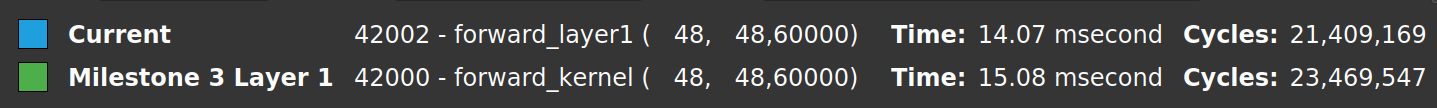
\includegraphics[width=\linewidth]{2kern_layer1_runtime}
        \caption{Execution Time}
    \end{subfigure}
    \begin{subfigure}[b]{\linewidth}
        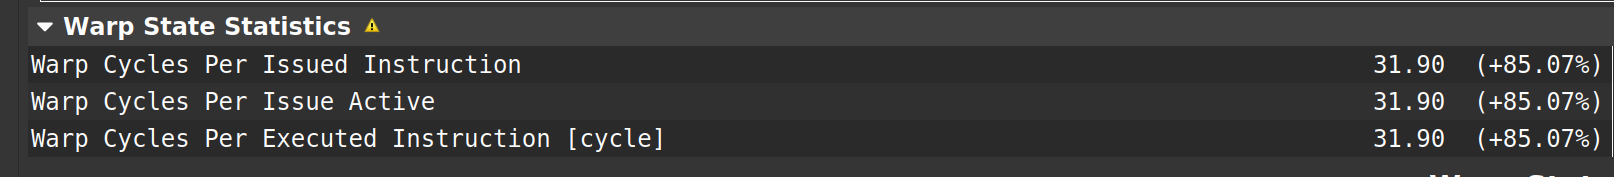
\includegraphics[width=\linewidth]{2kern_layer1_warp}
        \caption{Warp Statistics}
    \end{subfigure}
    \caption{Layer 1 Statistics}
\end{figure}

\begin{figure}[H]
    \centering
    \begin{subfigure}[b]{\linewidth}
        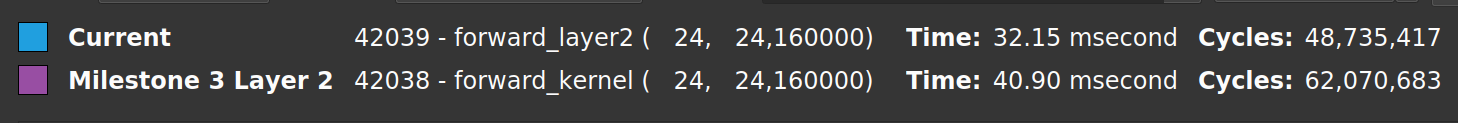
\includegraphics[width=\linewidth]{2kern_layer2_runtime}
        \caption{Execution Time}
    \end{subfigure}
    \begin{subfigure}[b]{\linewidth}
        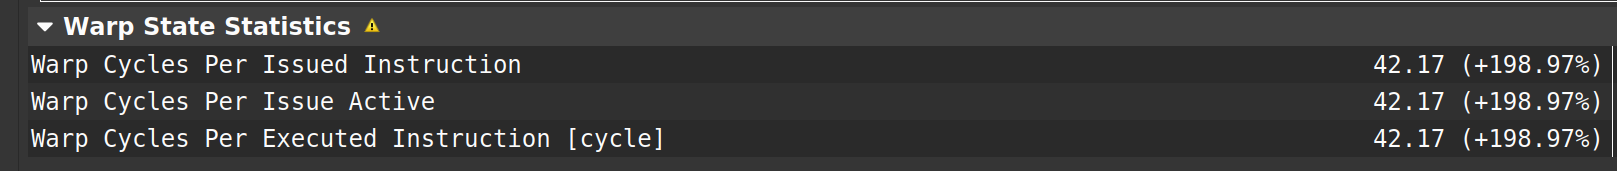
\includegraphics[width=\linewidth]{2kern_layer2_warp}
        \caption{Warp Statistics}
    \end{subfigure}
    \caption{Layer 2 Statistics}
\end{figure}

\paragraph{Note}
Now, we have already implemented different kernel functions for the two layers. Since optimizations in Section 2.1
are merely parameter tuning for each layer, we would like to directly implement further optimizations based
upon the two-kernel version in Section 2.1 and analyze the results by comparing to that version instead of
the original unoptimized version.

\subsection{Kernels in Constant Memory}
One optimization is to put kernels in constant memory by using
cudaMemcpyToSymbol() API call. This optimization is possible because convolution
kernels are
effectively read-only for each CUDA kernel launch. The contribution by this
optimization alone results in a relatively small amount of improvement in runtime
due to increasing efficiency of memory accessing throughput. The constant memory
kernel alone did not boost up too much the performance due to the bottleneck
of global memory fetching induced by the input element accesses.

\begin{figure}[H]
    \centering
    \begin{subfigure}[b]{\linewidth}
        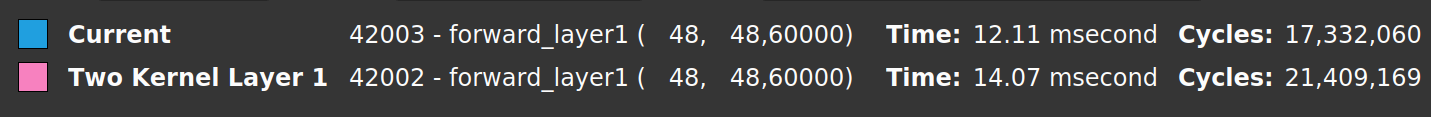
\includegraphics[width=\linewidth]{const_layer1_runtime}
        \caption{Execution Time}
    \end{subfigure}
    \begin{subfigure}[b]{\linewidth}
        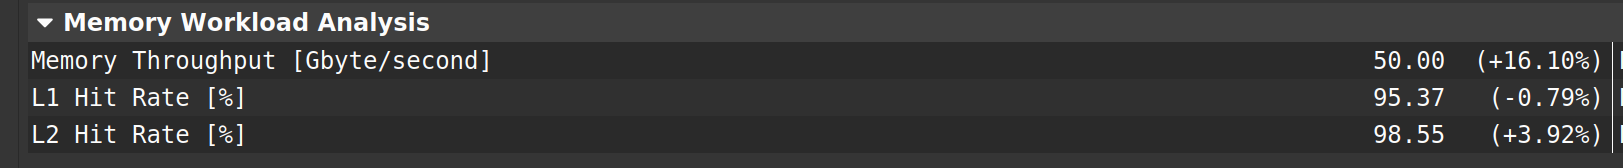
\includegraphics[width=\linewidth]{const_layer1_mem}
        \caption{Memory Throughput}
    \end{subfigure}
    \caption{Layer 1 Statistics}
\end{figure}

\begin{figure}[H]
    \centering
    \begin{subfigure}[b]{\linewidth}
        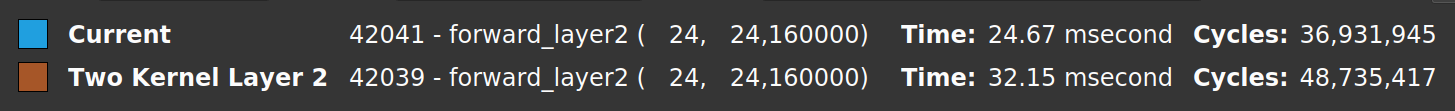
\includegraphics[width=\linewidth]{const_layer2_runtime}
        \caption{Execution Time}
    \end{subfigure}
    \begin{subfigure}[b]{\linewidth}
        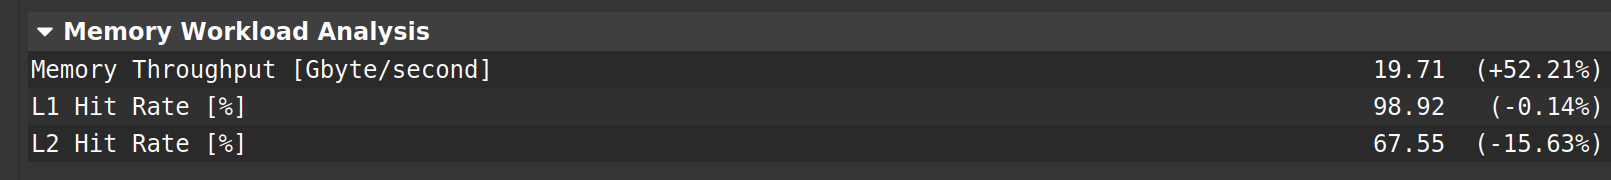
\includegraphics[width=\linewidth]{const_layer2_mem}
        \caption{Memory Throughput}
    \end{subfigure}
    \caption{Layer 2 Statistics}
\end{figure}


\subsection{Tiled Convolution using Shared Memory}
We can also optimize memory access pattern and reduce global memory access by caching
elements that are highly reused into shared memory for each thread block.
This optimization also implies that we break the input image into smaller tiles
and each thread block processes a tile of elements at one time. \\

\par
We chose loading strategy one, where all threads are utilized in multiple loop
cycles to load the slightly bigger shared tile of data. The reason for not using
strategy 2 is that we realize the finite computing resources is one of the
biggest limiting factor of performance, so we don't want to waste the extra threads
that are active only in loading stage but idle in computing stage. From the runtime
report below, we can see that this optimization alone did not improve too much
of the overall runtime, but even
slightly hurt the performance. This is because of the bottleneck presented
in reading the kernel data from global memory. Since the kernel is quite small,
many threads are competing for the same addresses which causes a lot of serialization
in the calculation loop. The tiled strategy, however, does introduce some overhead
in the loading stage. Despite all of these, the overall memory throughput is still
increased by this optimization.

\begin{figure}[H]
    \centering
    \begin{subfigure}[b]{\linewidth}
        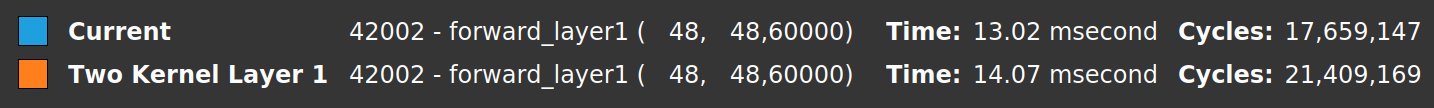
\includegraphics[width=\linewidth]{shared_layer1_runtime}
        \caption{Execution Time}
    \end{subfigure}
    \begin{subfigure}[b]{\linewidth}
        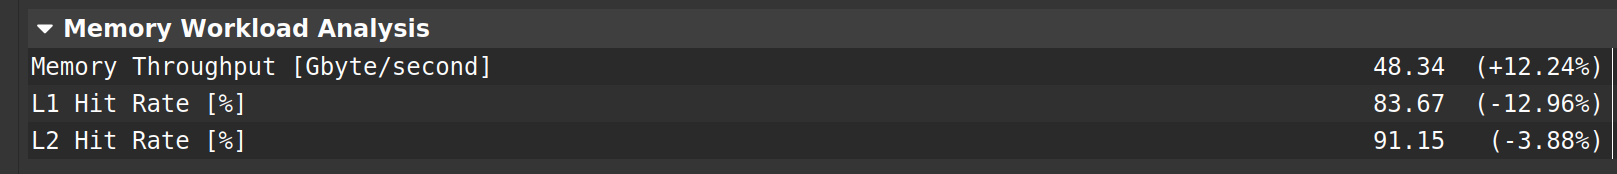
\includegraphics[width=\linewidth]{shared_layer1_mem}
        \caption{Memory Throughput}
    \end{subfigure}
    \caption{Layer 1 Statistics}
\end{figure}

\begin{figure}[H]
    \centering
    \begin{subfigure}[b]{\linewidth}
        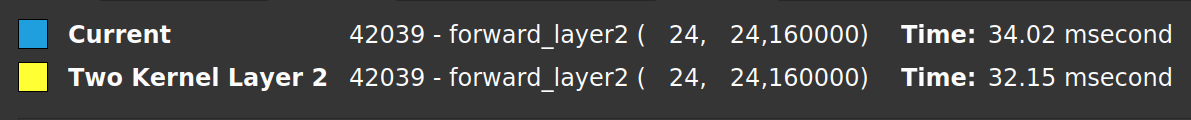
\includegraphics[width=\linewidth]{shared_layer2_runtime}
        \caption{Execution Time}
    \end{subfigure}
    \begin{subfigure}[b]{\linewidth}
        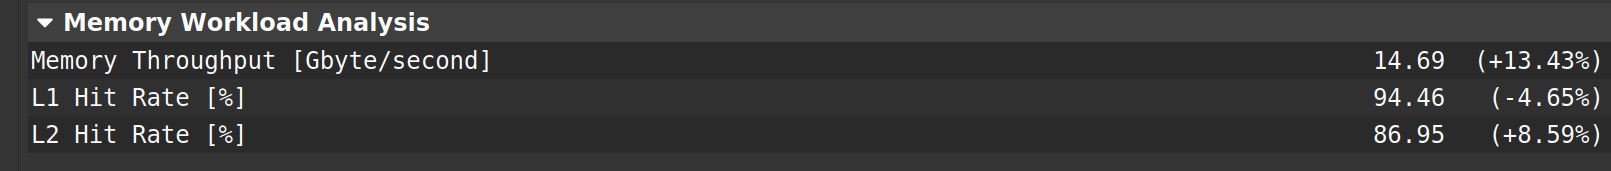
\includegraphics[width=\linewidth]{shared_layer2_mem}
        \caption{Memory Throughput}
    \end{subfigure}
    \caption{Layer 2 Statistics}
\end{figure}

\subsection{Combined Optimization}
Now we combine all the optimizations to benchmark against our Two Kernel baseline
implementation, we can see a great deal of improvement in runtime, memory throughput,
and SM occupancy. From the statistics below we can see that a lot less threads
are stalling for memory operations and more time are spent in floating point
computation. The combination of constant cached kernel and tiled convolution
completely takes away global memory access in the computing stage. And since shared
tile loading is almost perfectly coealesed with this linearized strategy, the
runtime is dramatically reduced.

\begin{figure}[H]
    \centering
    \begin{subfigure}[b]{\linewidth}
        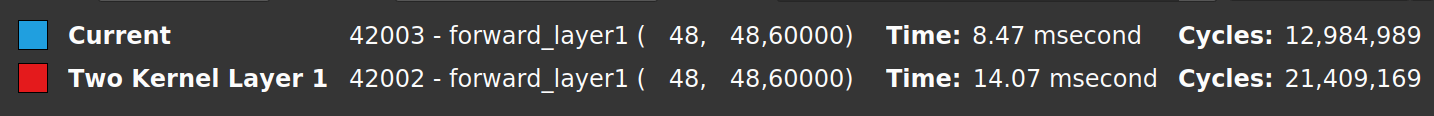
\includegraphics[width=\linewidth]{ms4_layer1_runtime}
        \caption{Execution Time}
    \end{subfigure}
    \begin{subfigure}[b]{\linewidth}
        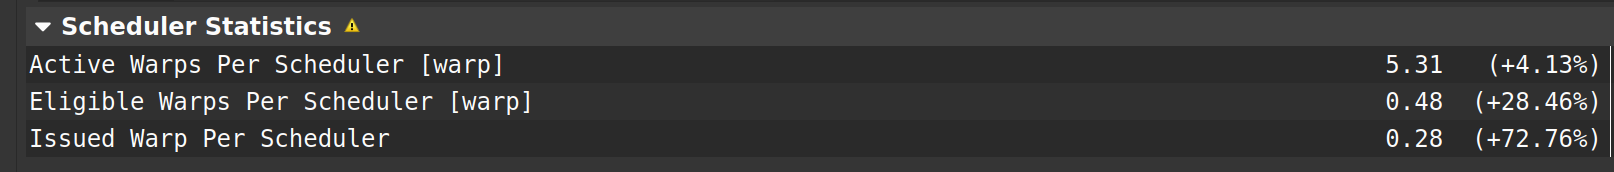
\includegraphics[width=\linewidth]{ms4_layer1_warp}
        \caption{Warp Statistics}
    \end{subfigure}
    \begin{subfigure}[b]{\linewidth}
        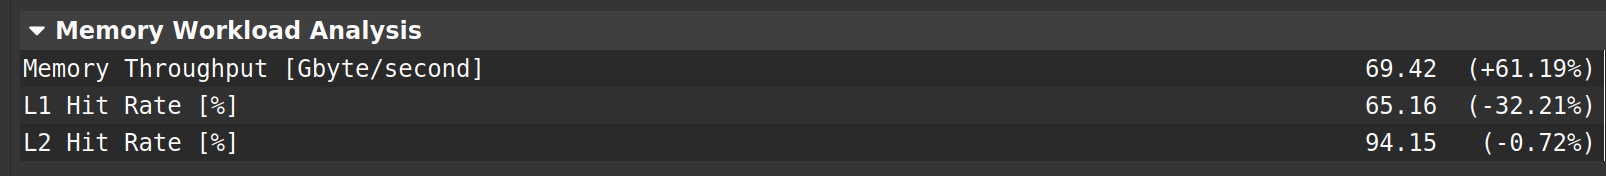
\includegraphics[width=\linewidth]{ms4_layer1_mem}
        \caption{Memory Throughput}
    \end{subfigure}
    \caption{Layer 1 Statistics}
\end{figure}

\begin{figure}[H]
    \centering
    \begin{subfigure}[b]{\linewidth}
        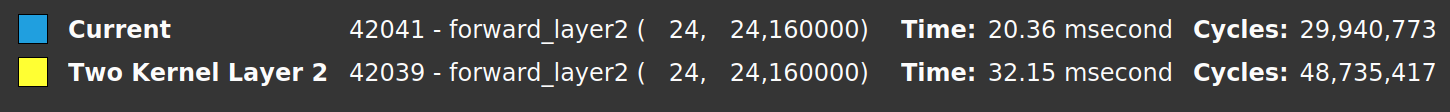
\includegraphics[width=\linewidth]{ms4_layer2_runtime}
        \caption{Execution Time}
    \end{subfigure}
    \begin{subfigure}[b]{\linewidth}
        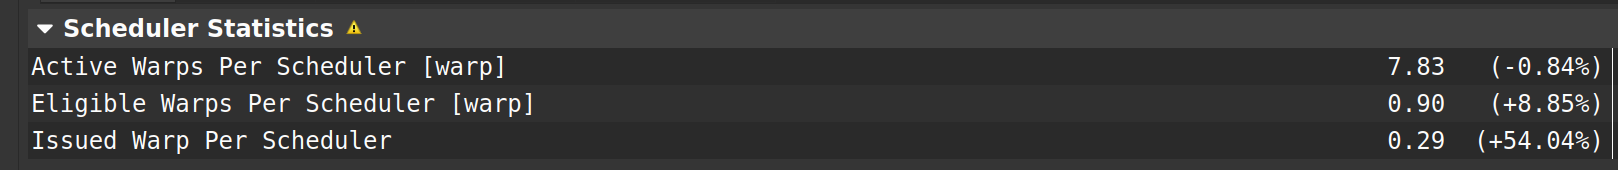
\includegraphics[width=\linewidth]{ms4_layer2_warp}
        \caption{Warp Statistics}
    \end{subfigure}
    \begin{subfigure}[b]{\linewidth}
        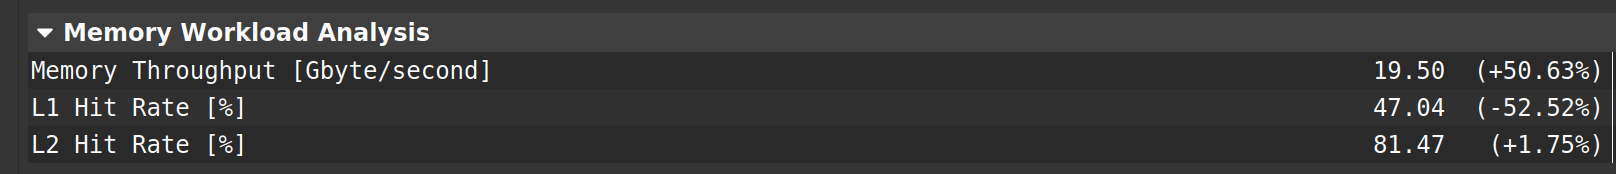
\includegraphics[width=\linewidth]{ms4_layer2_mem}
        \caption{Memory Throughput}
    \end{subfigure}
    \caption{Layer 2 Statistics}
\end{figure}

\part*{Milestone 5}
\setcounter{section}{0}

\section{Execution Summary}
Upon Milestone 5, we have implemented three additional optimizations to our feed-forward
convolution kernel. The optimizations include loop unrolling, pointer restriction with
\verb|const| and \verb|__restrict__| quantifier, parameter tunning, register-shared caching, and half precision acceleration.
All of the optimization combined help us reduce the run time by a factor of 1/5.
Below is a summary of the execution runtime and accuracy on the server.

\begin{table}[H]
    \centering
    \begin{minipage}{.32\linewidth}
        \begin{tabular}{c|c}
            Accuracy & 0.8397 \\ \hline
            First Layer Time & 1.053ms \\ \hline
            Second Layer Time & 1.509ms
        \end{tabular}
        \caption*{10000 images}
    \end{minipage}
    ~
    \begin{minipage}{.32\linewidth}
        \begin{tabular}{c|c}
            Accuracy & 0.852 \\ \hline
            First Layer Time & 0.147ms \\ \hline
            Second Layer Time & 0.251ms
        \end{tabular}
        \caption*{1000 images}
    \end{minipage}
    ~
    \begin{minipage}{.32\linewidth}
        \begin{tabular}{c|c}
            Accuracy & 0.84 \\ \hline
            First Layer Time & 0.070ms \\ \hline
            Second Layer Time & 0.099ms
        \end{tabular}
        \caption*{100 images}
    \end{minipage}
    \caption{Run time statistics after applying all three optimizations.}
\end{table}

\section{Optimizations}

\paragraph{Note}
Same as in Milestone 4, we would like to mention that, in order to avoid unexpected server fluctuations and speedup our development,
we have setup a local development environment using an NVIDIA GeForce RTX 2080 running CUDA 10.0. Our discussions below will be based on
execution results and statistics generated in our local environment. Despite this, we have ensured that our optimizations work as
intended on the server. Also, for simplicity, we will only benchmark data size 10000.

\subsection{Parameter Tunning with Loop Unrolling \& Pointer Restriction}

\textbf{Note.} Parameter Tunning is disccussed in the next section as we changed
the overall program logic in it. As a result, parameter tunning is based on
the new excution pattern in the next optimization.\\

\textbf{Motivation.} Since our threads are mapped to the output matrix elements,
each threads will require iterations to accumulate for the convolution result.
The boundary check overhead is not negligible when the loop is nested as well as
when the iteration size is large. So, loop unrolling can help eliminate those overhead
and improve runtime. Moreover, it can also help save registers as the loop indices
are no longer required.\\

\textbf{Result.} As this is comparing against our milestone 4 baseline, which is
a rather naive implementation of the kernel, loops are not quite deep, and there
are other bottlenecks such as memory throughput, so loop unrolling does not actually
provide too much of a performance increase. But in general, we can still see some
expected behavior in terms of register usage and runtime. In addition to that,
the warp starts to spend more time stalling on memory operations, as the index generation
overhead is reduced. The benifit of the loop unrolling is
much more obvious for later optimizations as the complexity of iterations grows bigger.\\

\begin{figure}[H]
    \centering
    \begin{subfigure}[b]{\linewidth}
        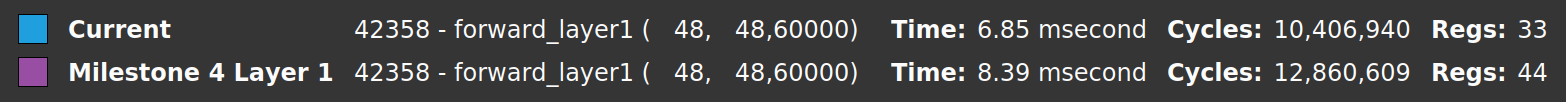
\includegraphics[width=\linewidth]{pragma_layer1_summary}
        \caption{Execution Time}
    \end{subfigure}
    \begin{subfigure}[b]{\linewidth}
        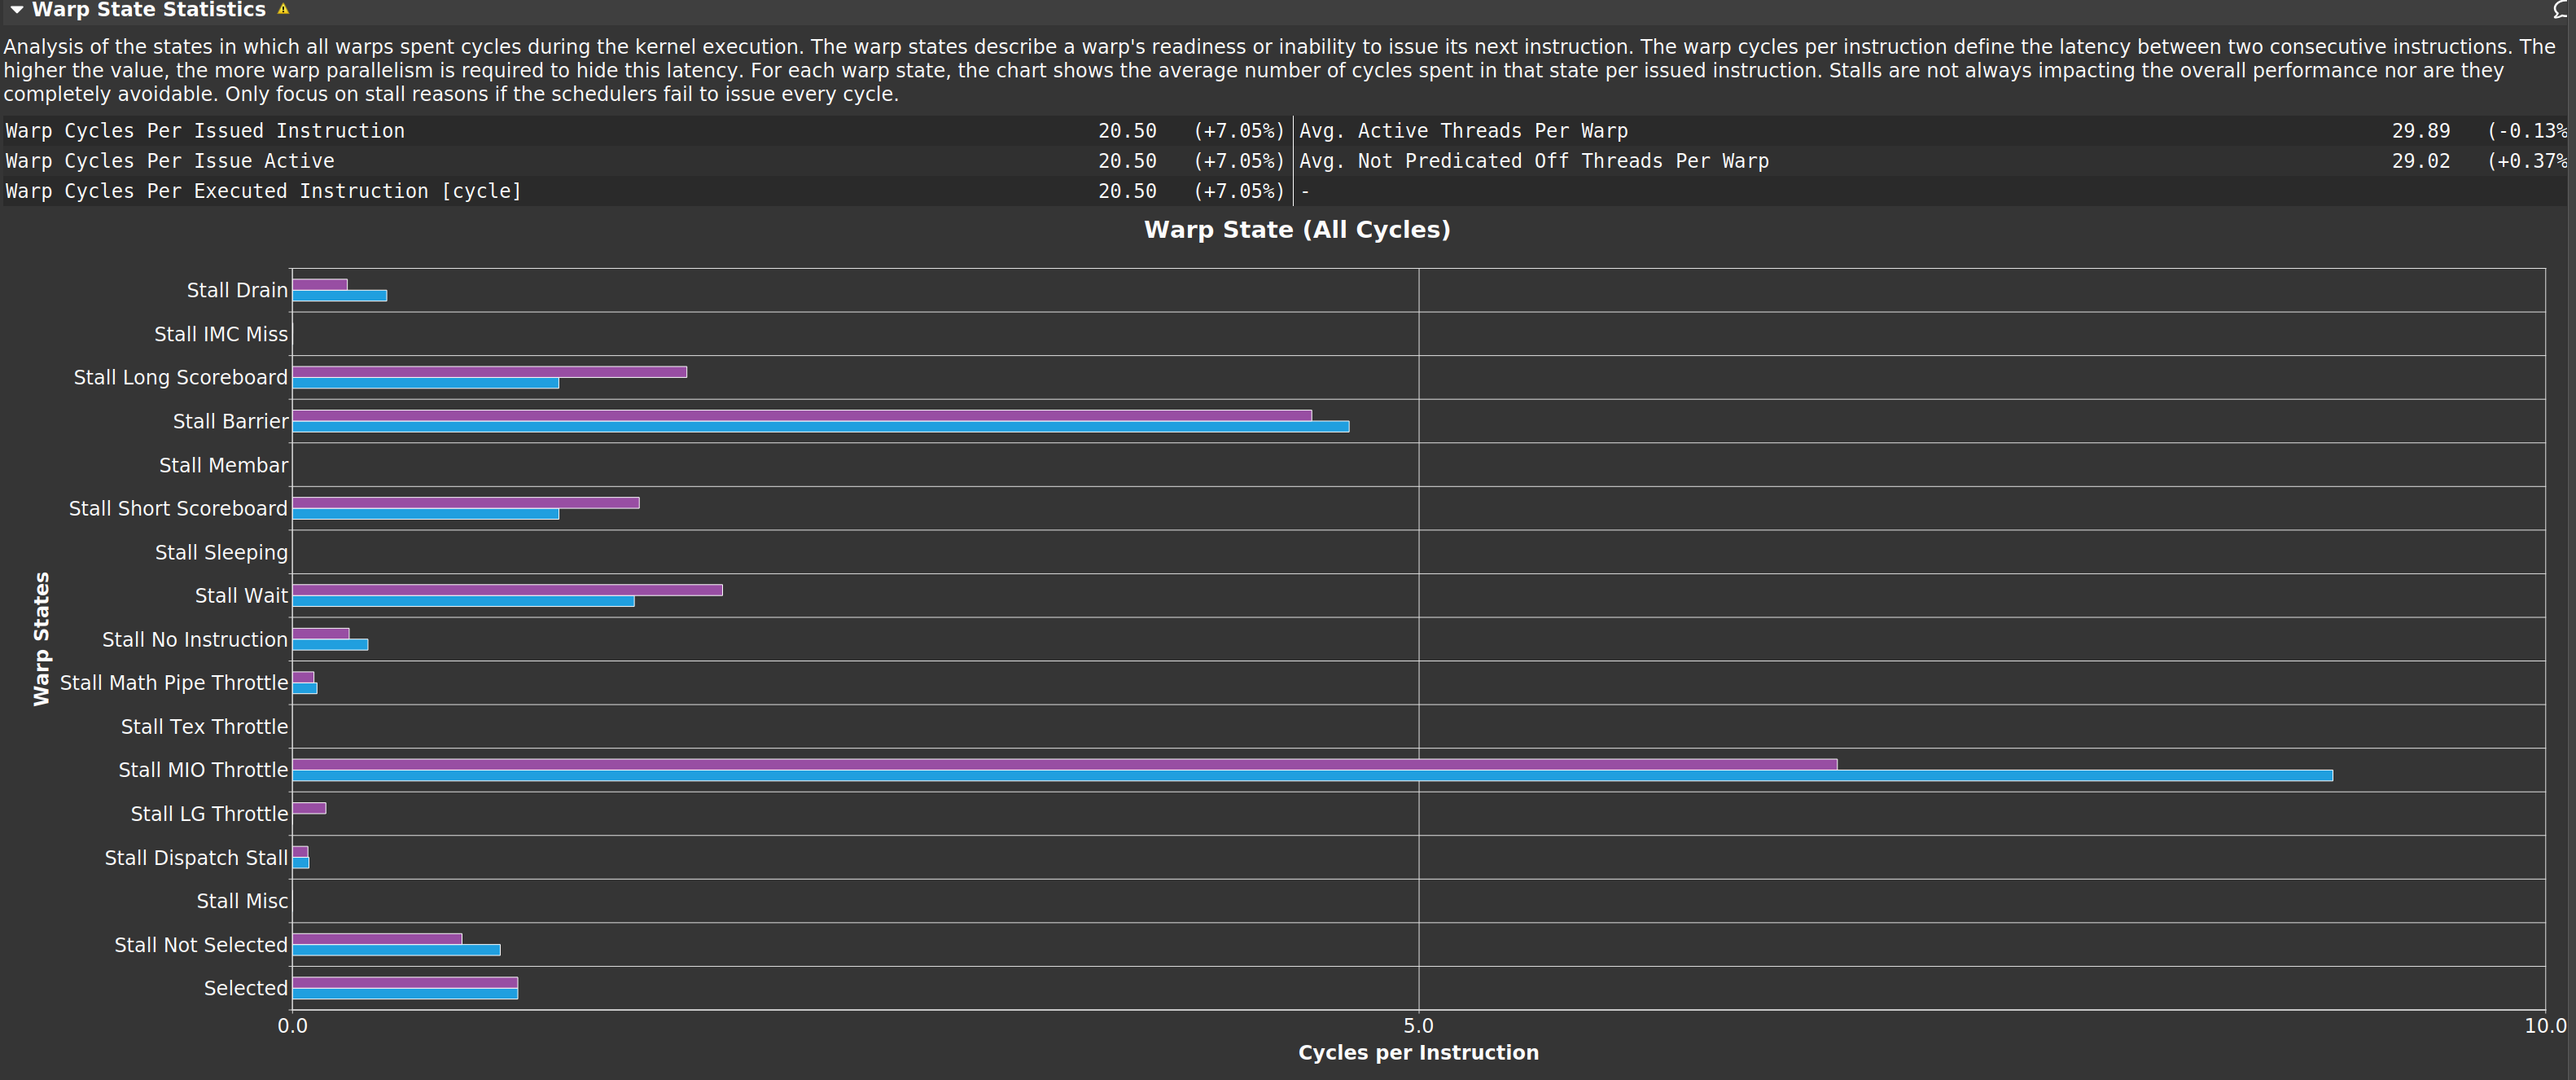
\includegraphics[width=\linewidth]{pragma_layer1_warp}
        \caption{Warp Stall Reasons}
    \end{subfigure}
    \caption{Layer 1 Statistics}
\end{figure}

\begin{figure}[H]
    \centering
    \begin{subfigure}[b]{\linewidth}
        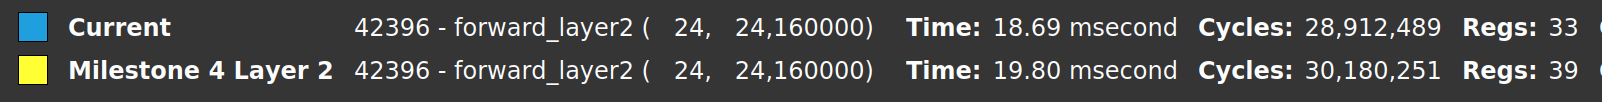
\includegraphics[width=\linewidth]{pragma_layer2_summary}
        \caption{Execution Time}
    \end{subfigure}
    \begin{subfigure}[b]{\linewidth}
        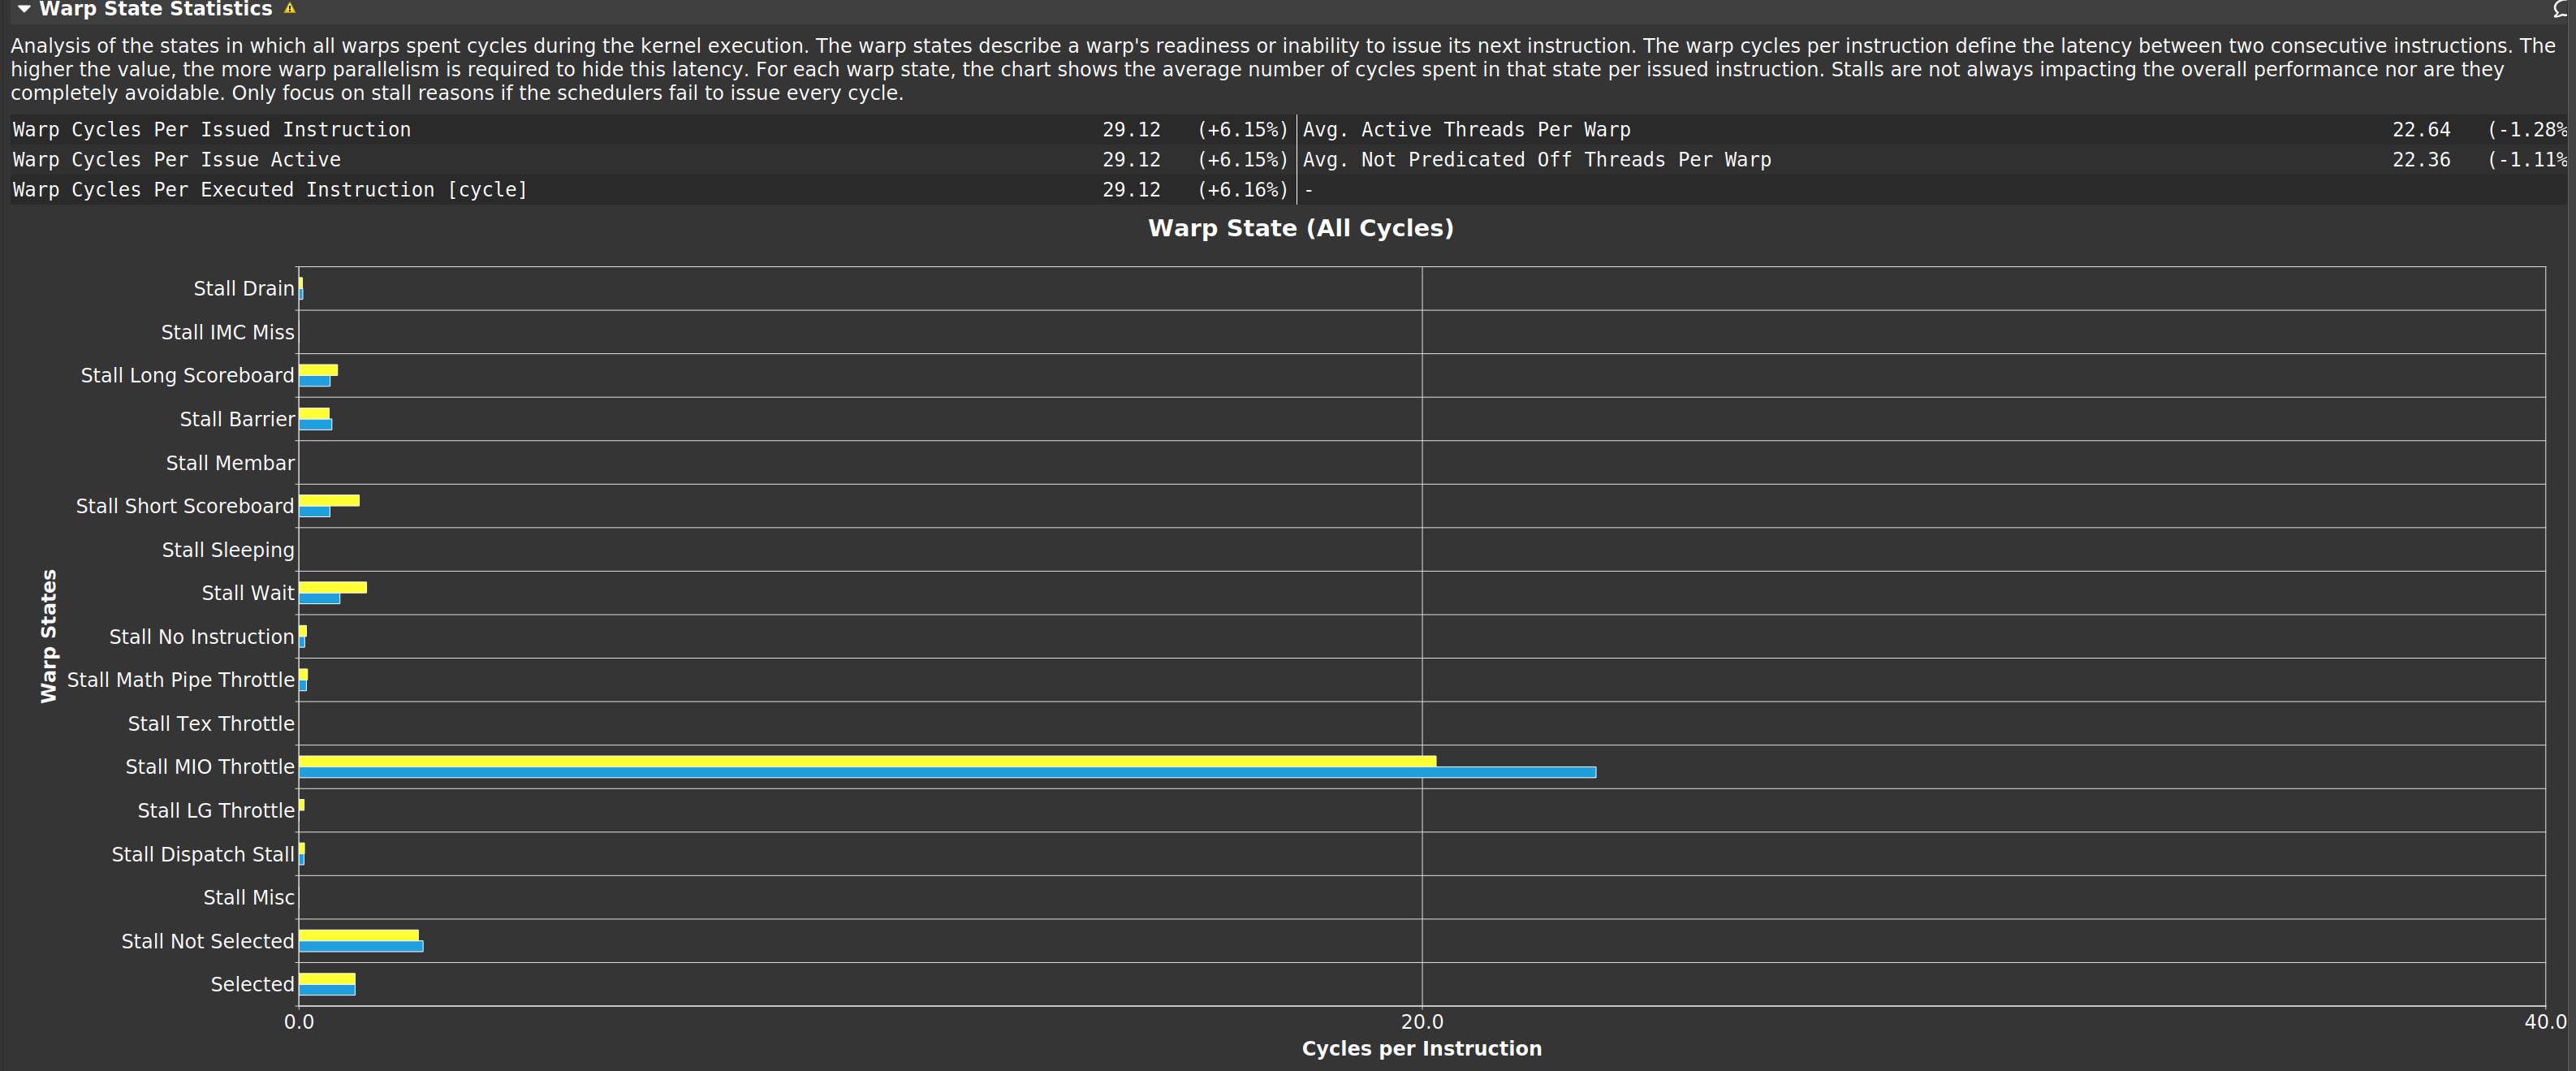
\includegraphics[width=\linewidth]{pragma_layer2_warp}
        \caption{Warp Stall Reasons}
    \end{subfigure}
    \caption{Layer 2 Statistics}
\end{figure}

\subsection{Register-Shared Caching}
\textbf{Motivation.} Though we have implemented shared-memory convolution,
we still observed that there are bottlenecks at memory throughput. By a thorough
investigation, we found that we can further reduce redundant shared-memory accesses
and optimize global memory access pattern by caching the most-reused data in
per-thread registers. This optimization is made possible thanks to the powerful
hardware provided by modern technologies (which ensures enough registers for us to
utilize) and the fact that we changed the thread mapping so that now each thread
calculates an output for each output feature map iteratively, i.e. for layer 1 which
we have 6 output feature maps, each thread calculates 6 outputs. This fact implies
that each thread would reuse elements in input feature maps for calculations of all
output feature maps. Hence, we could cache these reused elements in local registers
to improve shared-memory access efficiency. In addition to caching inputs, we also
cache output elements in local registers and write the results together to the
global memory after all calculations to ensure a coealesed write pattern. We expect
this to improve global memory write throughput.\\

\textbf{Parameter Tuning.} We tuned several parameters (especially kernel launch
configurations) after implementing register-shared caching (in fact, we almost
did such kind of tuning every time after a new optimization). In the case of
this optimization that implements register-shared caching, we made a significant
change to memory access pattern by configuring a non-square thread block.
Specifically, we take layer 1 as an example, which has one $48\times48$ input feature map and six $44\times44$ output feature maps. Since the input and output
elements are organized linearly in memory, we can use a $11\times44$ tile to match
the organization of the output elements. As we expected, we observed a great deal
of increase in memory access efficiency and significant decrease in run time after
applying this configuration. \\

\textbf{Result.} This optimization is the most significant one among all three.
From the benchmark, we could see it provides a 4x increase in overall performance.
If we analyze further into the details, we could see the memory throughput
increased a lot for both layers. The shared computing scheme results in a lot less
shared memory accesses as well as constant memory cache misses. The memory throughput
is increased around 3x for both layers as indicated in the figure below. From the
warp statistic section, we also see that the Stall MIO (Memory IO) is reduced by
a great factor that the kernel no longer have a significant stalling source. If
we look into the instruction statistics, it is also very obvious that this optimization
saves a lot of duplicated executions for both memory fetch and computations.

\begin{figure}[H]
    \centering
    \begin{subfigure}[b]{\linewidth}
        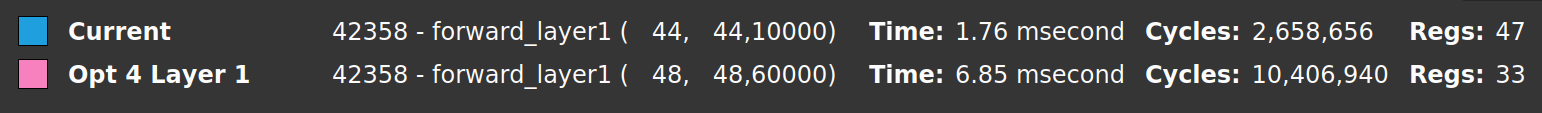
\includegraphics[width=\linewidth]{reg_share_layer1_summary}
        \caption{Execution Time}
    \end{subfigure}
    \begin{subfigure}[b]{\linewidth}
        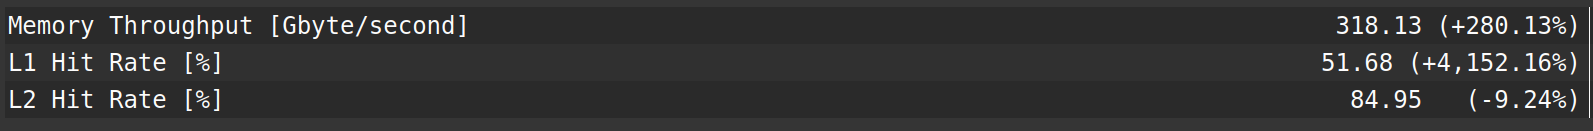
\includegraphics[width=\linewidth]{reg_share_layer1_mem}
        \caption{Memory Throughput}
    \end{subfigure}
    \begin{subfigure}[b]{\linewidth}
        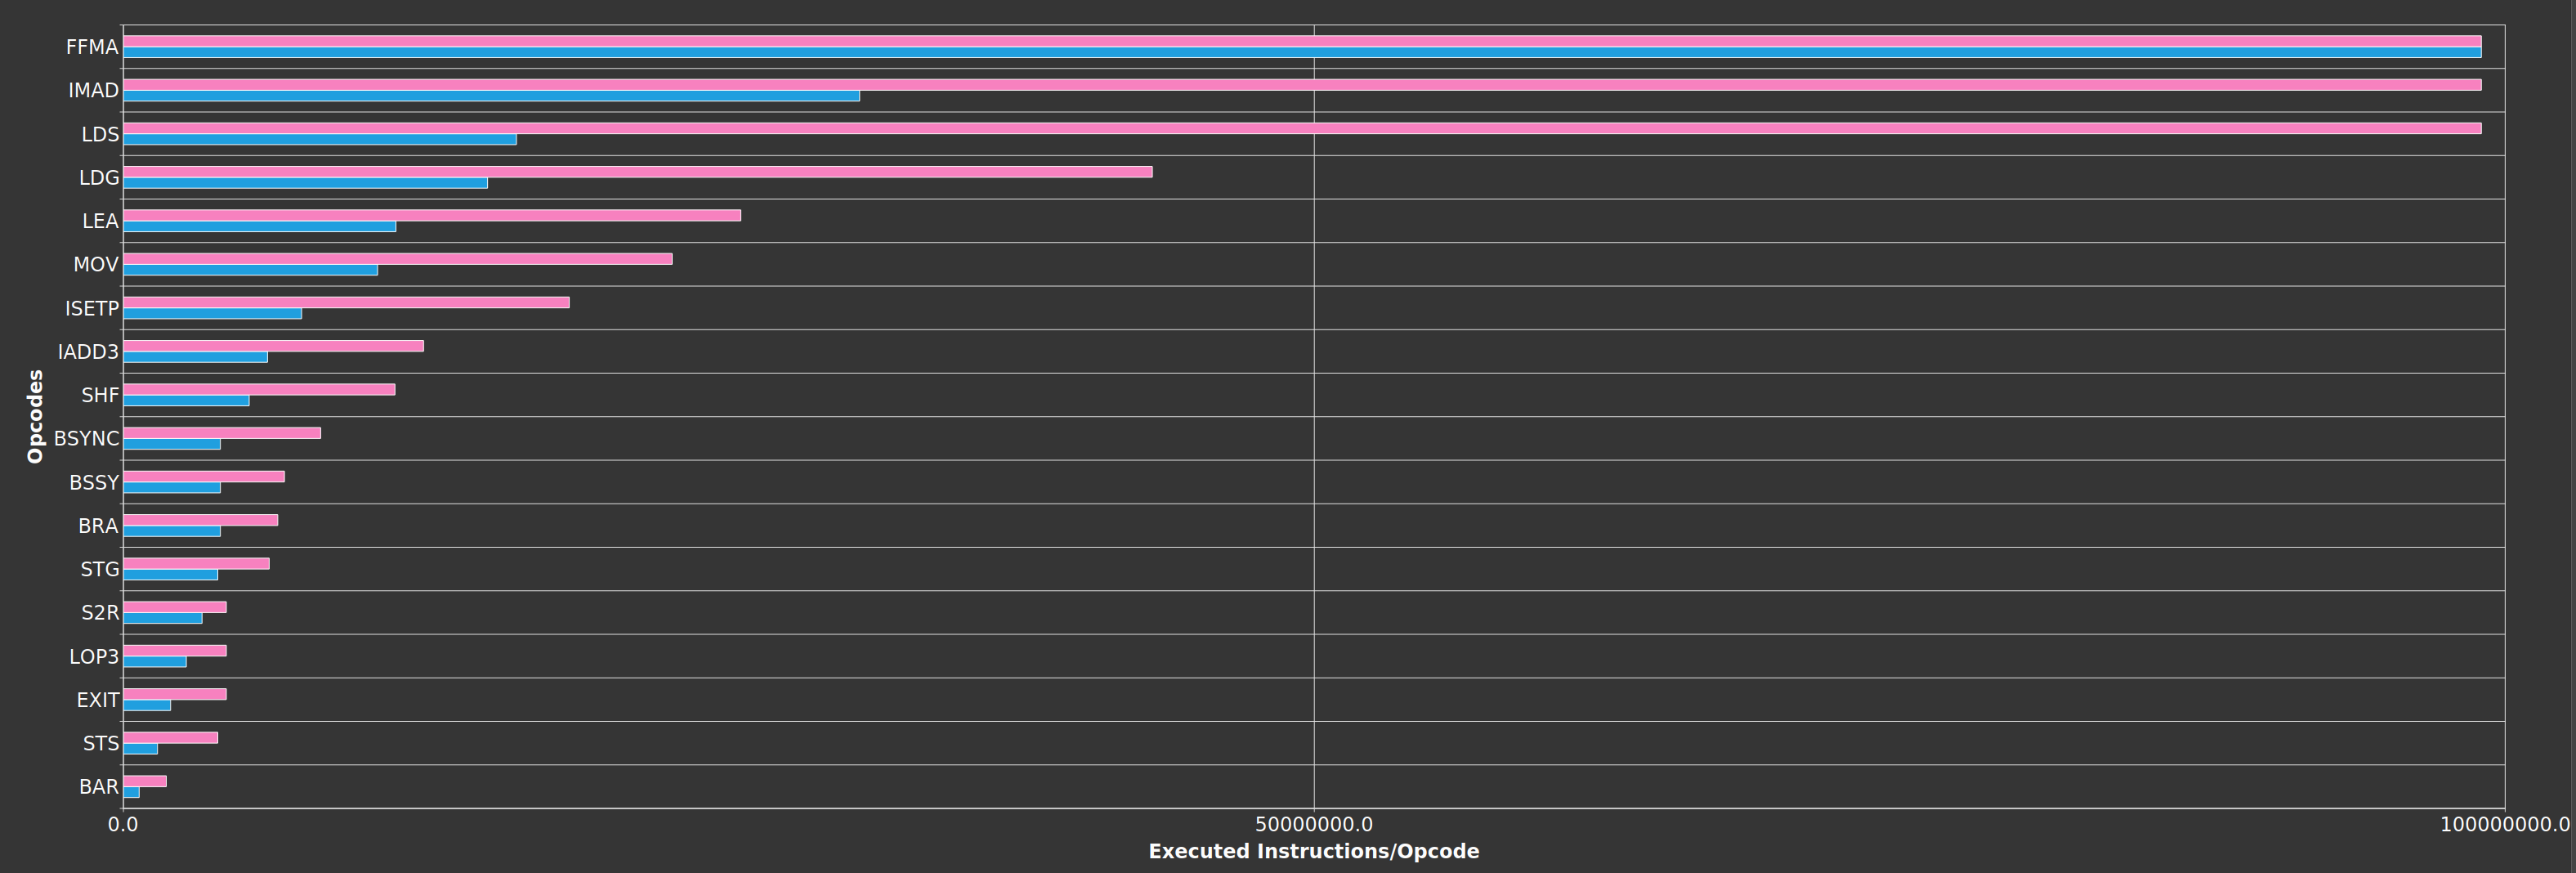
\includegraphics[width=\linewidth]{reg_share_layer1_opcode}
        \caption{Instruction Statistics}
    \end{subfigure}
    \begin{subfigure}[b]{\linewidth}
        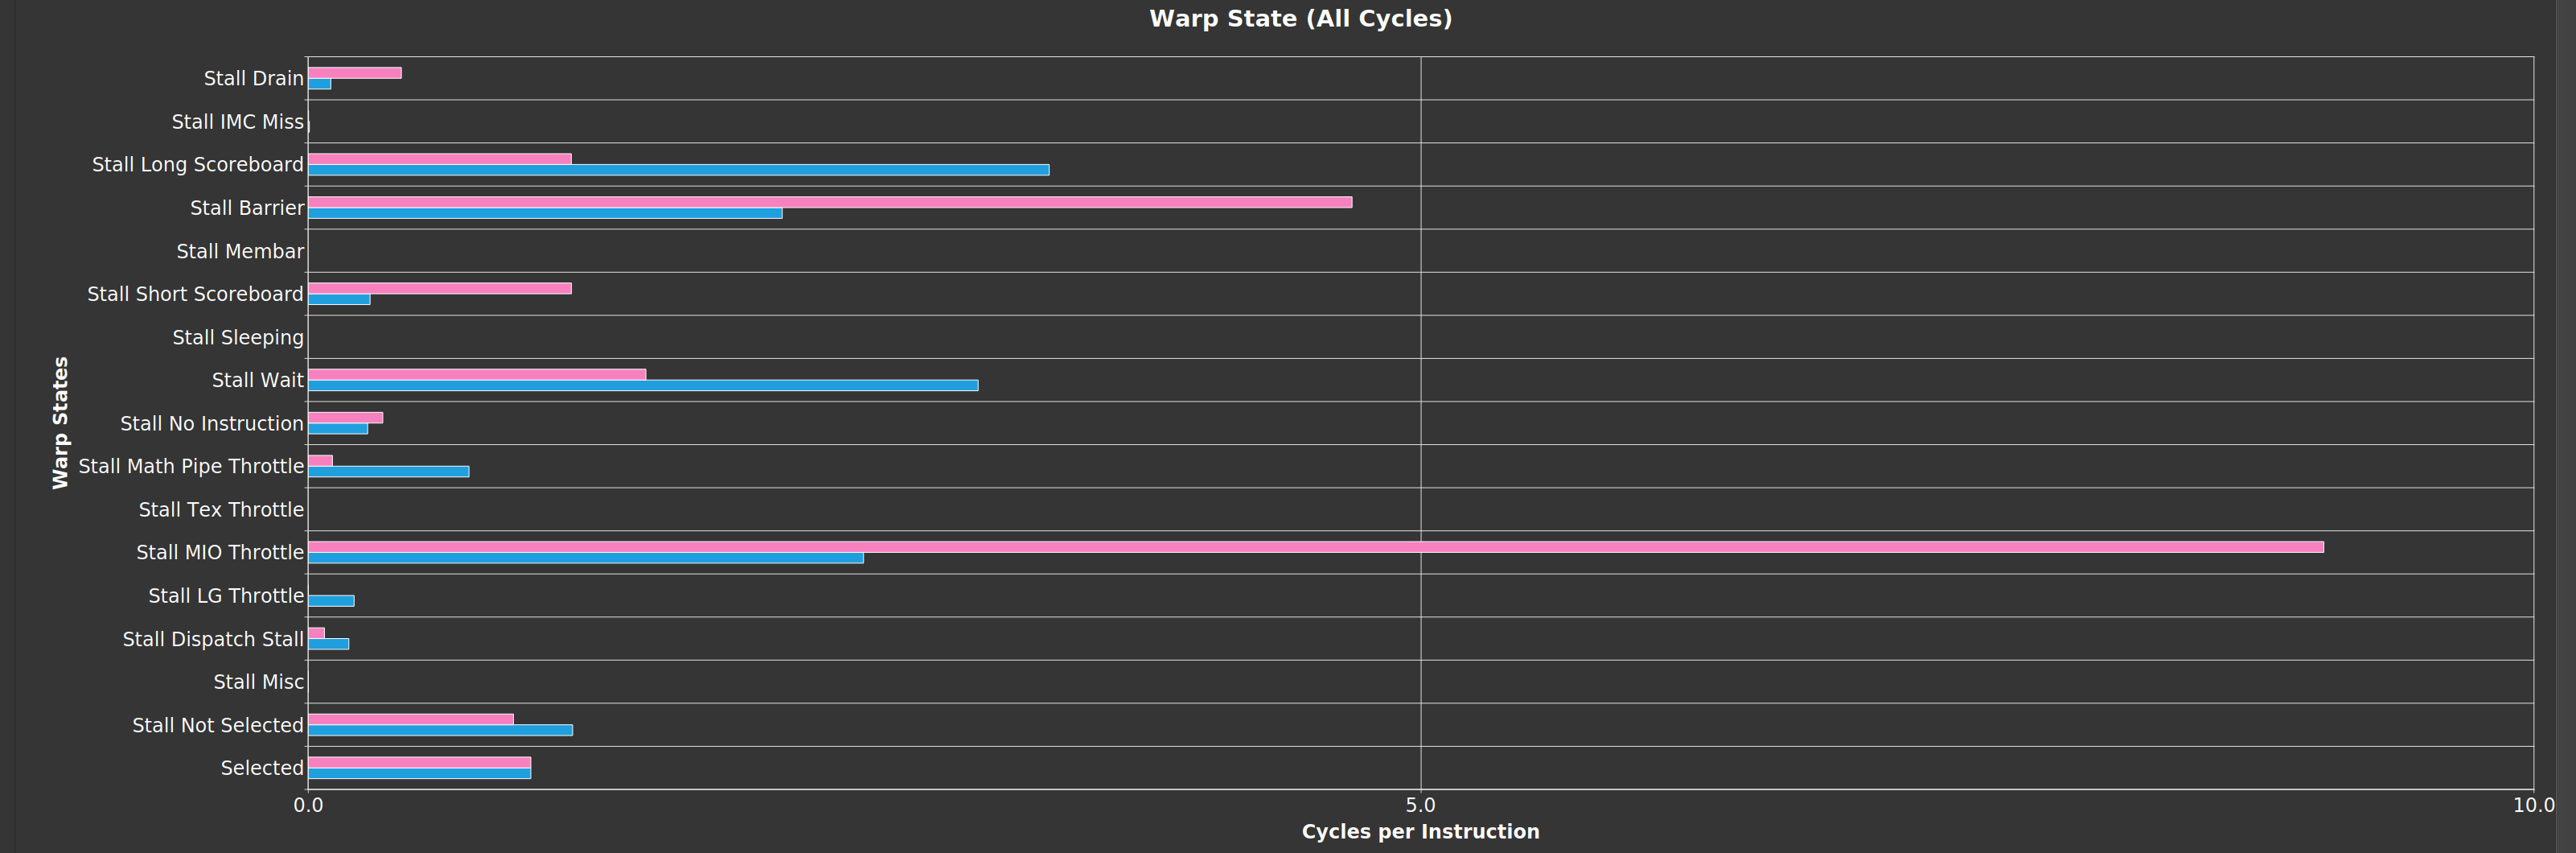
\includegraphics[width=\linewidth]{reg_share_layer1_warp}
        \caption{Stall Reasons}
    \end{subfigure}
    \caption{Layer 1 Statistics}
\end{figure}

\begin{figure}[H]
    \centering
    \begin{subfigure}[b]{\linewidth}
        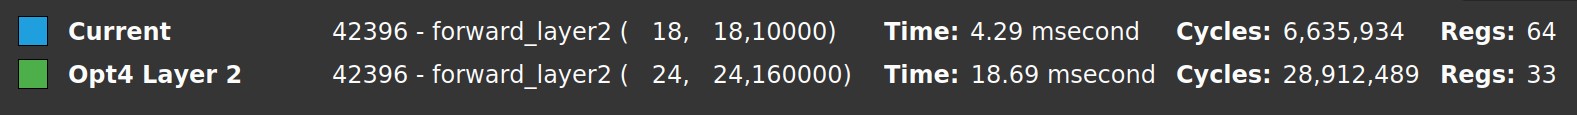
\includegraphics[width=\linewidth]{reg_share_layer2_summary}
        \caption{Execution Time}
    \end{subfigure}
    \begin{subfigure}[b]{\linewidth}
        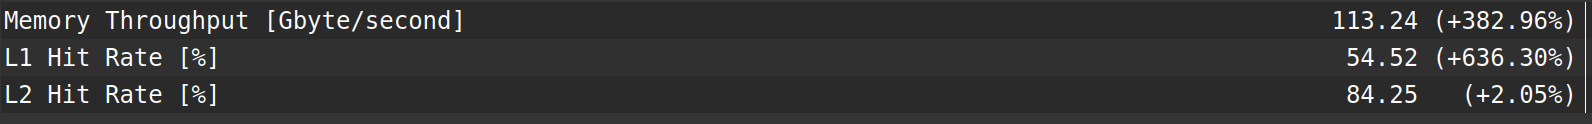
\includegraphics[width=\linewidth]{reg_share_layer2_mem}
        \caption{Memory Throughput}
    \end{subfigure}
    \begin{subfigure}[b]{\linewidth}
        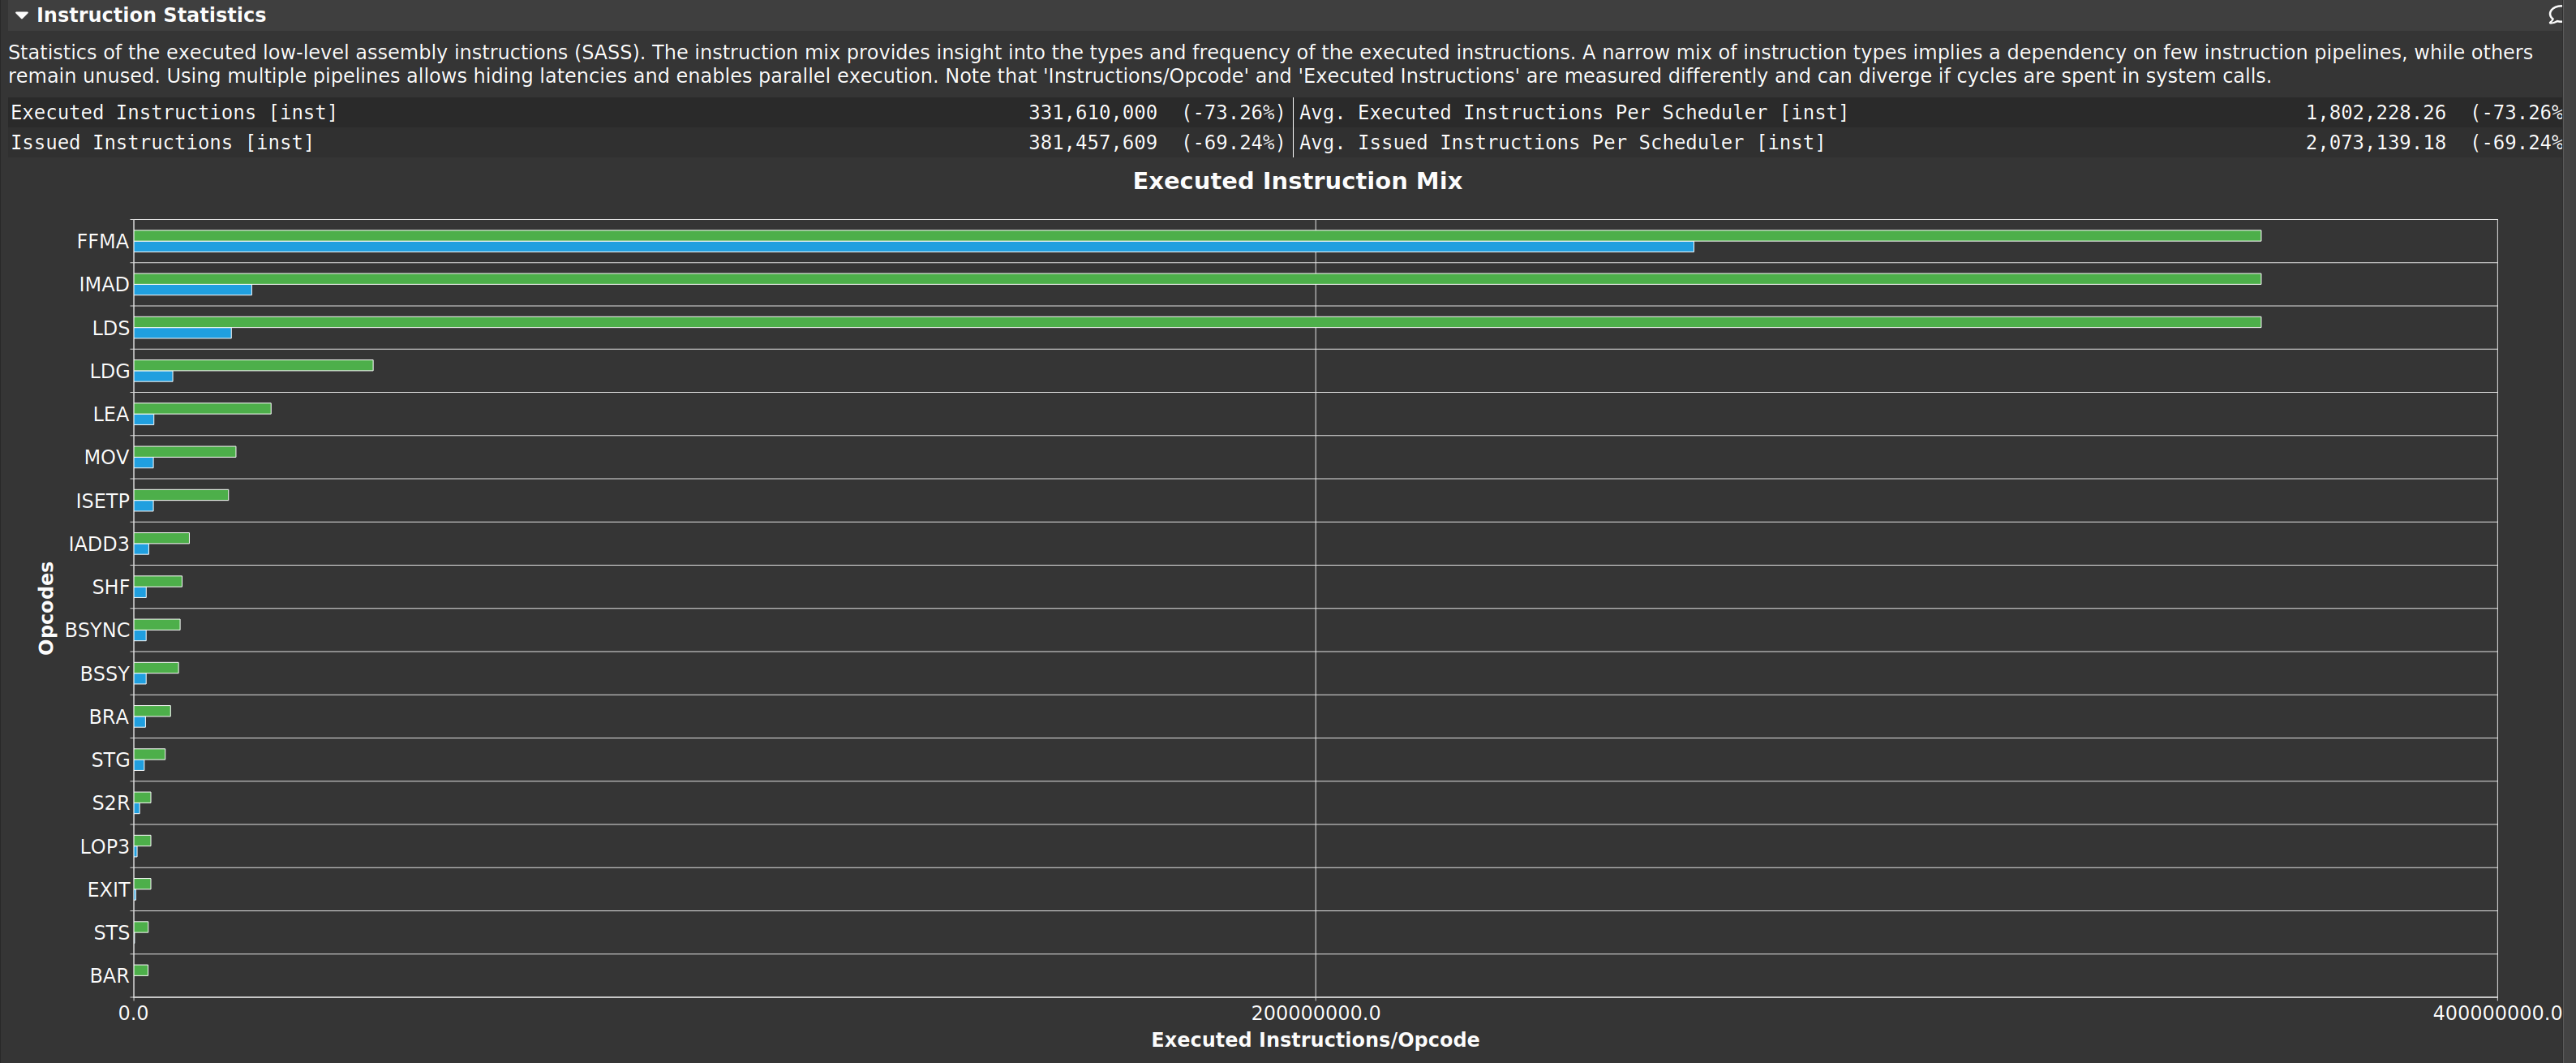
\includegraphics[width=\linewidth]{reg_share_layer2_opcode}
        \caption{Instruction Statistics}
    \end{subfigure}
    \begin{subfigure}[b]{\linewidth}
        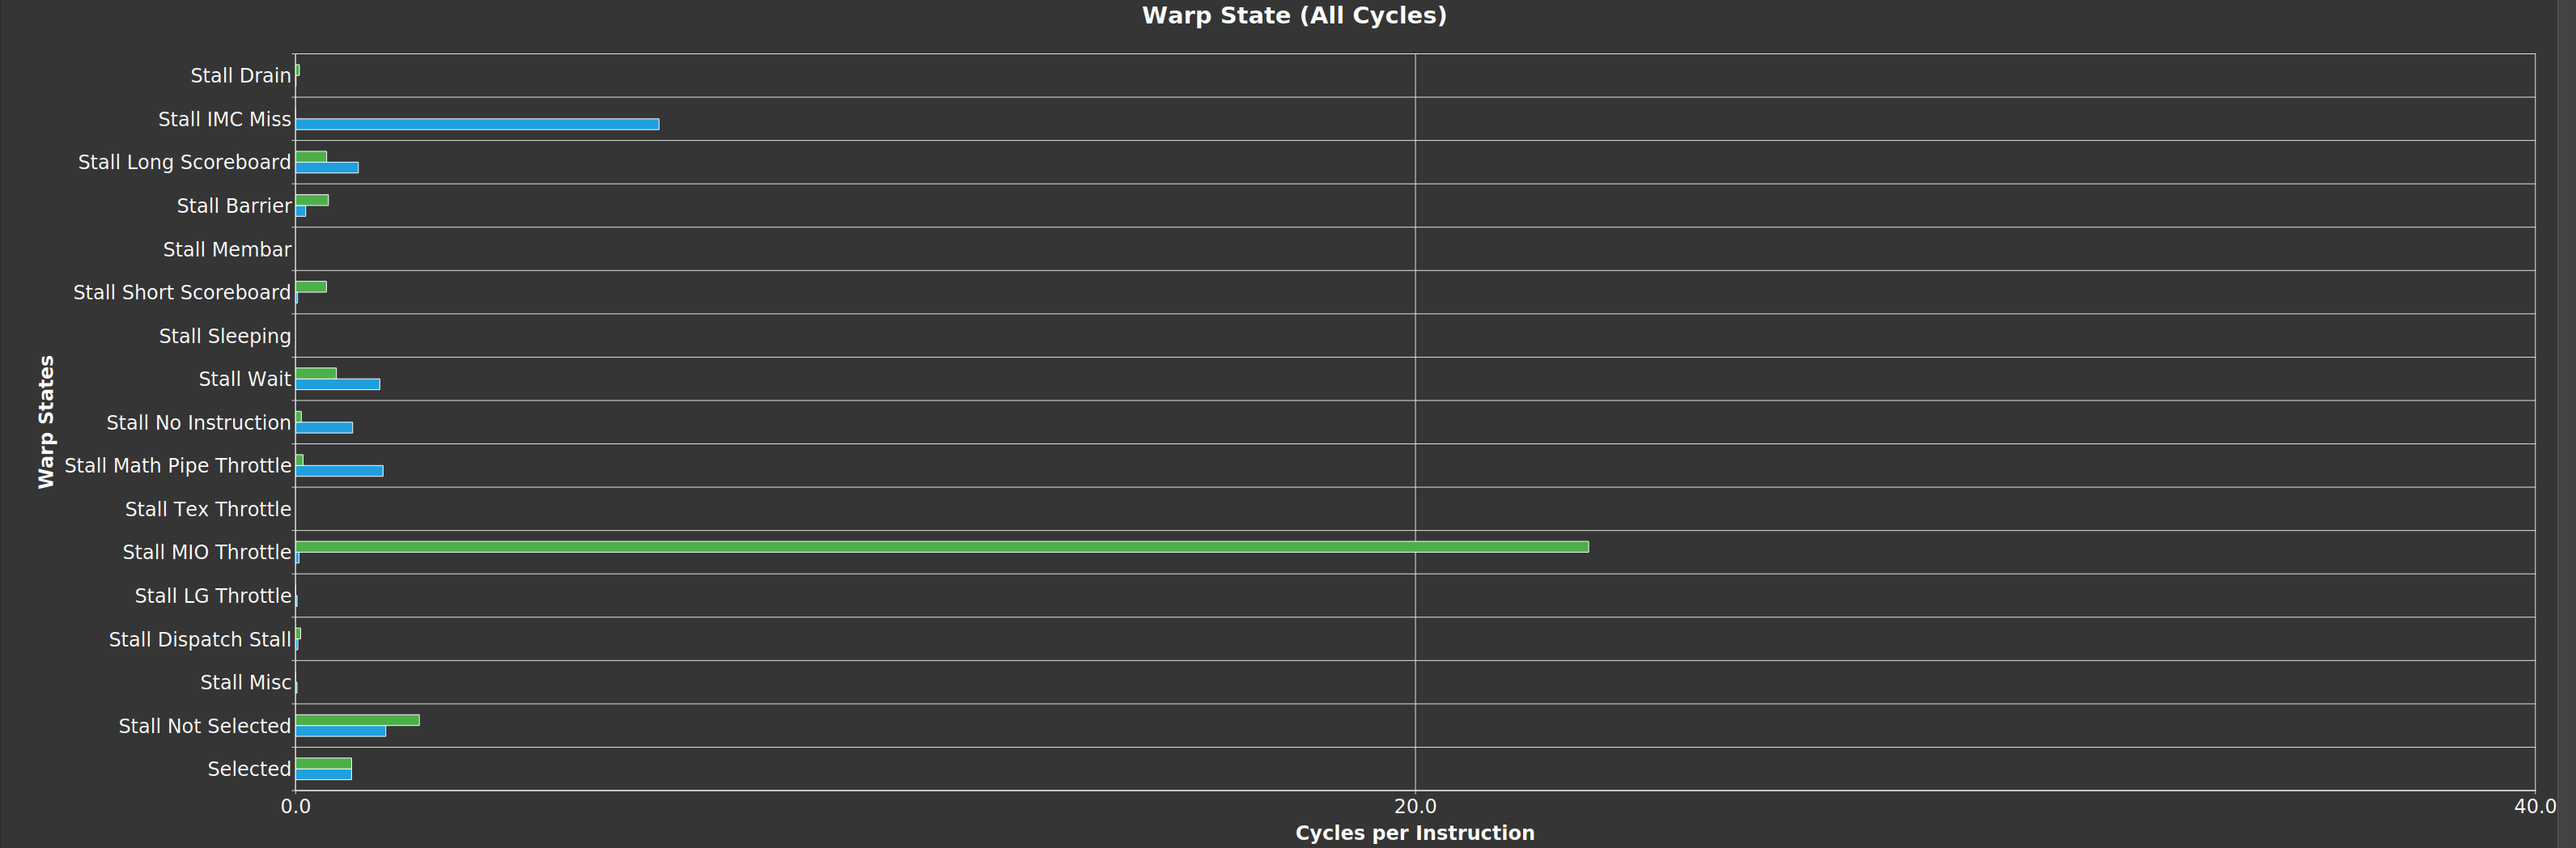
\includegraphics[width=\linewidth]{reg_share_layer2_warp}
        \caption{Stall Reasons}
    \end{subfigure}
    \caption{Layer 2 Statistics}
\end{figure}

\subsection{Half-Precision Arithmetic}
\textbf{Motivation.} After applying all of the previous optimizations, we found
it difficult to further improve from the perspective of algorithms, as we have
almost achieved the ideal thread occupacy and memory throughput in previous
optimizations. Since the essential arithmetic operation in our convolution
algorithm is FMA (Fused Multiplication and Addition) of floating-point numbers,
and multipling two 32-bit numbers should theoratically require a 64-bit number
to store the result (while we only have 32 bits), we considered an optimization
that replaces floating-point FMA by half-presicion-floating-point FMA. Particulally,
our CUDA device (and that one on the server) provides hardwares to do two
half-precision FMAs at one time. This would theoratically double the computation
throughput.\\

\textbf{Side Notes.} Here we only perform this half precision optimization for
layer 2. The main reason is that after a thorough analysis on the previous optimization
checkpoint, we found out that the performance of layer 2 is more limited by computation,
while layer 1 is more limited by memory. Therefore, our experiments revealed that implementing the half precision kernel
for layer 1 did not provide as much increase in performance as in layer 2, but also
introduced non-negligible overhead in launching another kernel to convert the constant
kernel weights to \verb|half2| data type.\\

\textbf{Result.} A very important detail of our implementation is that we utilized
the \verb|half2| arithmetic operations instead of just \verb|half| operations. This is because
CUDA hardward favors single \verb|half2| arithmetic over 2 \verb|half| instructions. In addition,
\verb|half2| (4-Byte) access in memory also follows a coealesed pattern for global memory
and bank-conflict-free pattern for shared memory. Therefore, memory throughput is
greatly increased with \verb|half2| data type. We split the output channel to 2 halves, so that
the x and y element of each \verb|half2| value contains the first and second half of the original
matrix elements. In terms of computation, according to NVIDIA's
documentation, \verb|half2| operations is almost as fast as \verb|float|
operations, so the computation time is theoratically reduced by a factor of 2 as only
half of the original threads are need where each of them compute twice as many output
elements. Since this optimization requires \verb|half2| type kernel as well, it
reduces the the overall size of the constant kernel. This is especially significant for layer 2
as the kernel size is quite large. The decrease in this kernel size also helps reduces the
constant cache misses when reading the constant weights.
The figure below confirmed the increase in runtime and memory throughput,
which results in an overall 2x increase in performance.

\begin{figure}[H]
    \centering
    \begin{subfigure}[b]{\linewidth}
        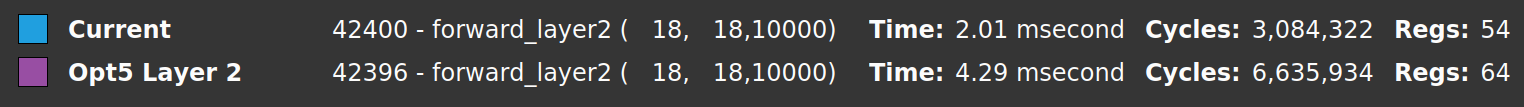
\includegraphics[width=\linewidth]{half_layer2_summary}
        \caption{Execution Time}
    \end{subfigure}
    \begin{subfigure}[b]{\linewidth}
        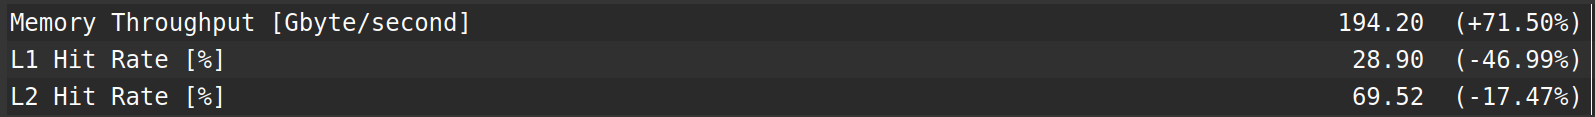
\includegraphics[width=\linewidth]{half_layer2_mem}
        \caption{Memory Throughput}
    \end{subfigure}
    \begin{subfigure}[b]{\linewidth}
        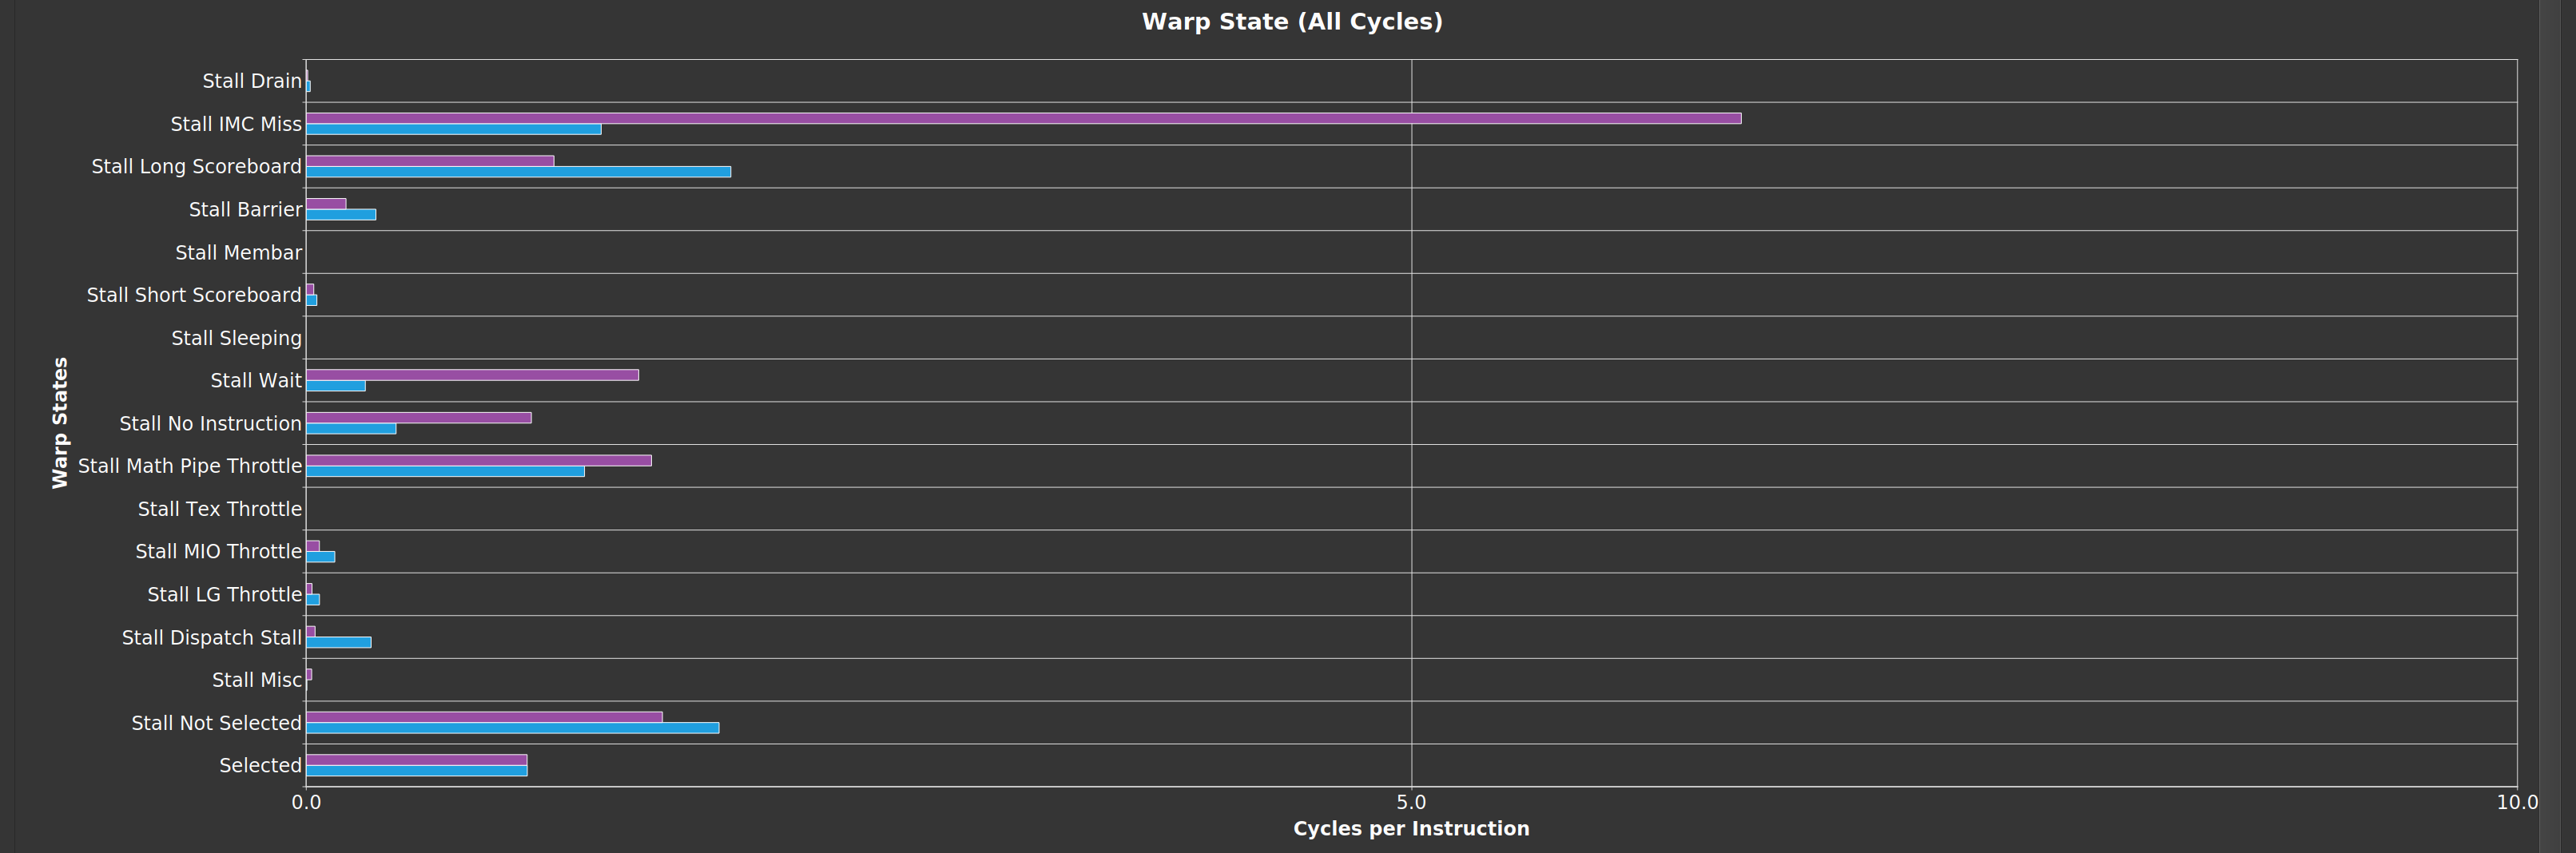
\includegraphics[width=\linewidth]{half_layer2_warp}
        \caption{Stall Reasons}
    \end{subfigure}
    \caption{Layer 2 Statistics}
\end{figure}

\subsection{Combined Optimization}
Now we combine all the optimizations in milestone 5 to benchmark against our
final version from milestone 4. The figures below indicated most of the major performance
metrics. The most straight forward one will be the runtime and memory throughput as they
are both improved by quite a big factor. However, a less obvious but important one is
how the total number of instructions is reduced. This metric can well confirm our
parallel logic reduced a great number of redundant operations with the latest 3
additional optimizations.

\begin{figure}[H]
    \centering
    \begin{subfigure}[b]{\linewidth}
        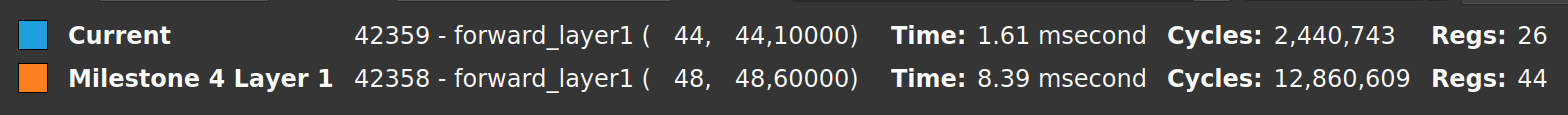
\includegraphics[width=\linewidth]{final_layer1_summary}
        \caption{Execution Time}
    \end{subfigure}
    \begin{subfigure}[b]{\linewidth}
        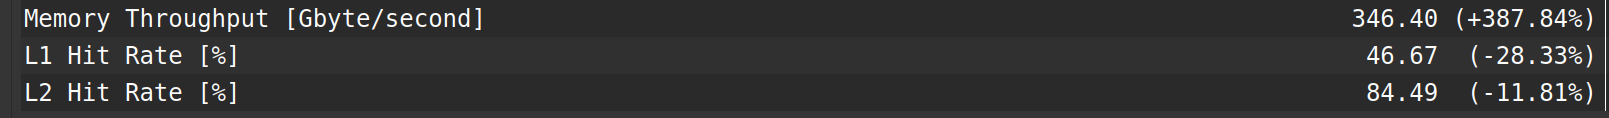
\includegraphics[width=\linewidth]{final_layer1_mem}
        \caption{Memory Throughput}
    \end{subfigure}
    \begin{subfigure}[b]{\linewidth}
        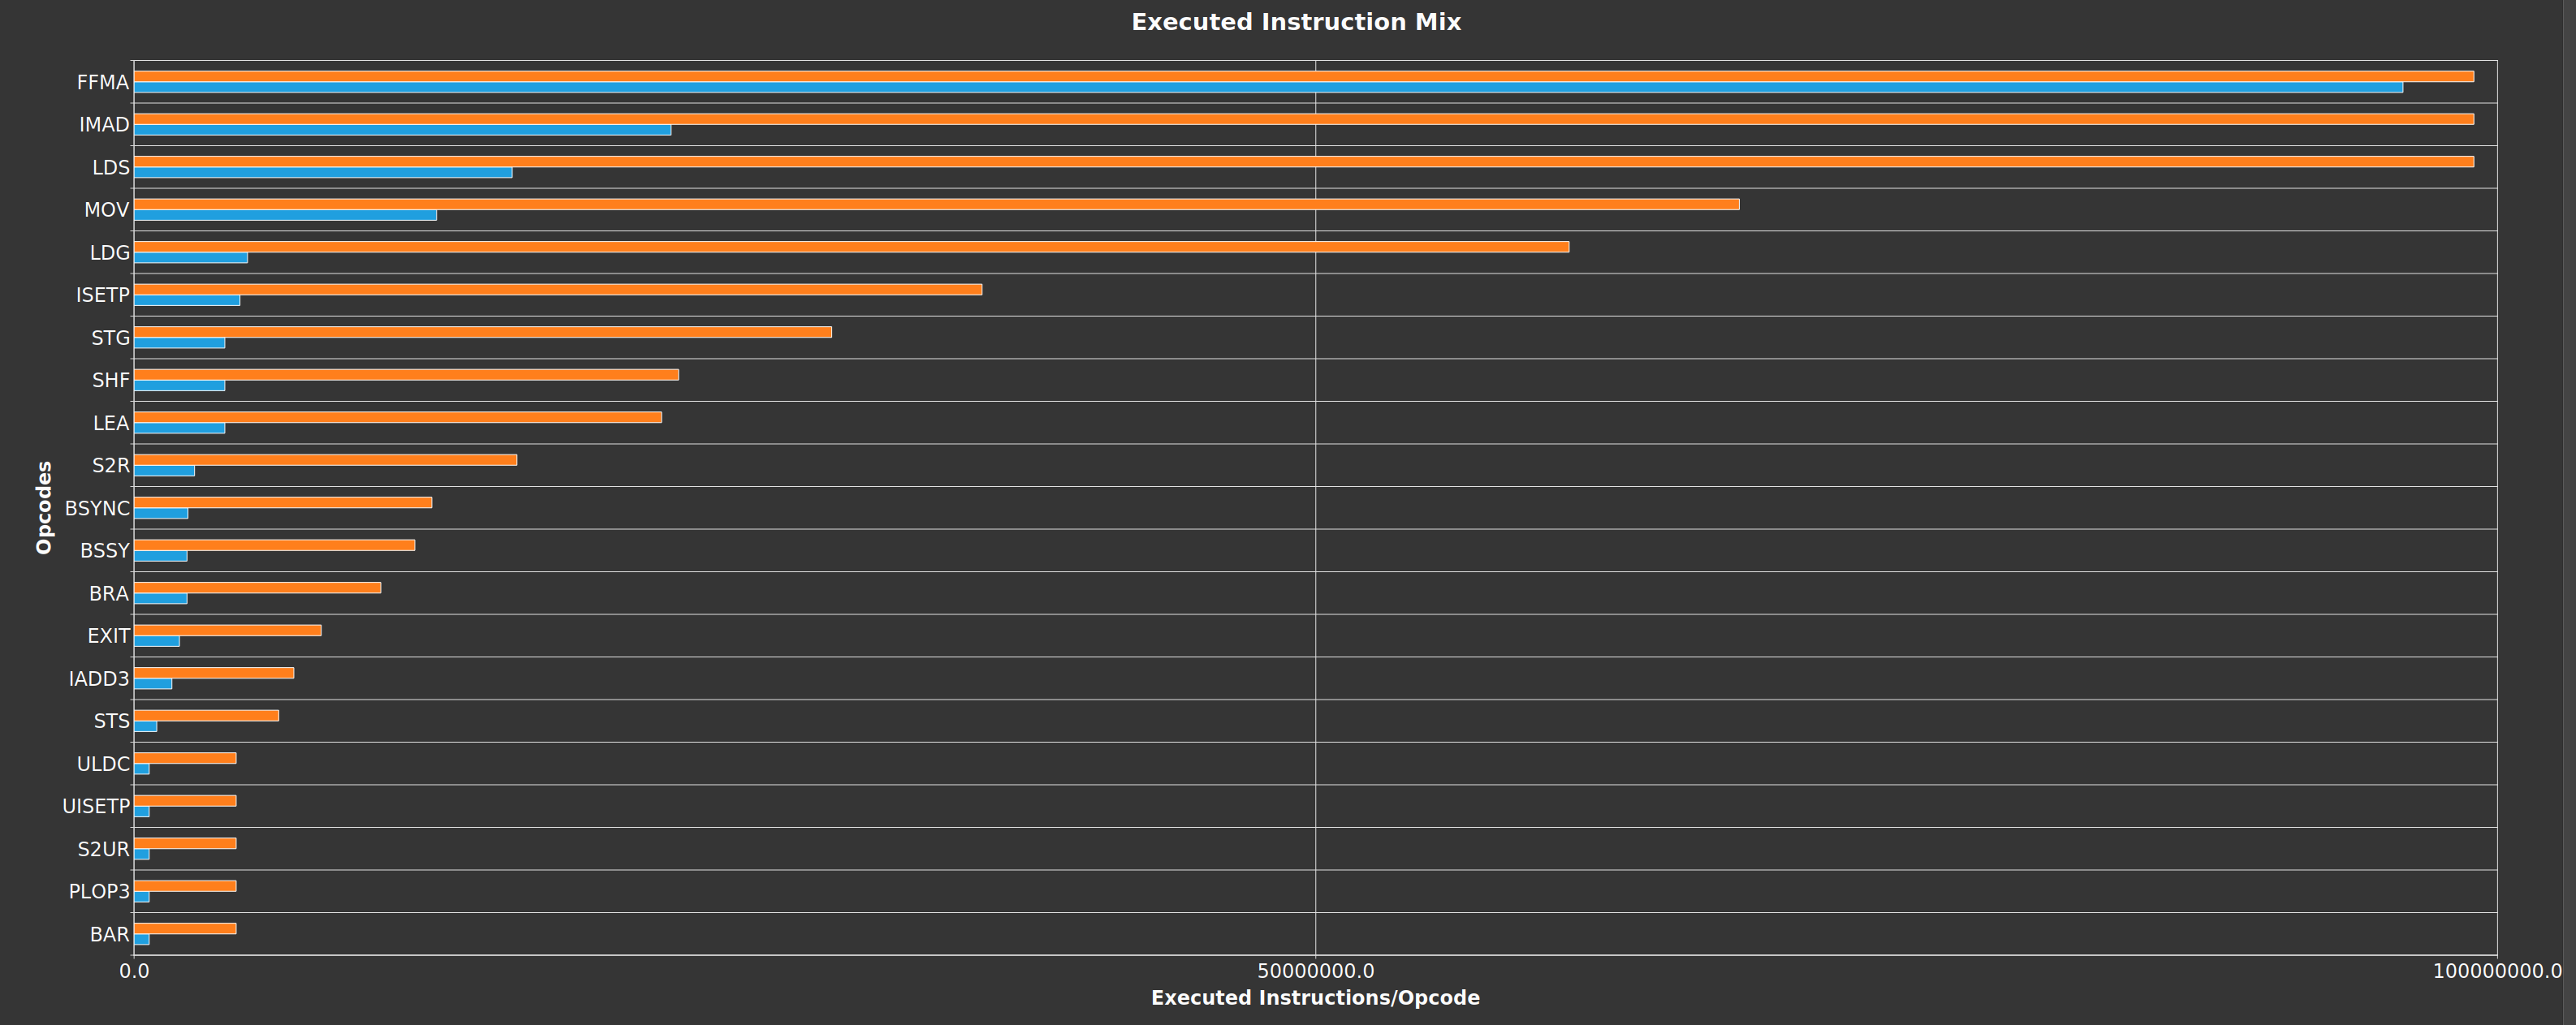
\includegraphics[width=\linewidth]{final_layer1_opcode}
        \caption{Stall Reasons}
    \end{subfigure}
    \caption{Layer 1 Statistics}
\end{figure}

\begin{figure}[H]
    \centering
    \begin{subfigure}[b]{\linewidth}
        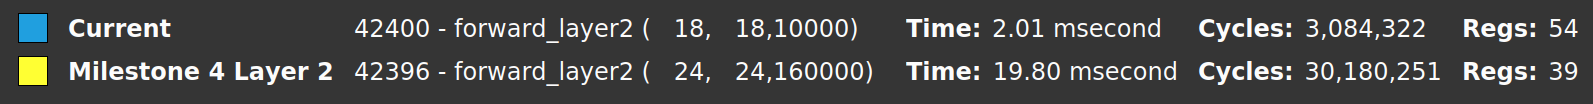
\includegraphics[width=\linewidth]{final_layer2_summary}
        \caption{Execution Time}
    \end{subfigure}
    \begin{subfigure}[b]{\linewidth}
        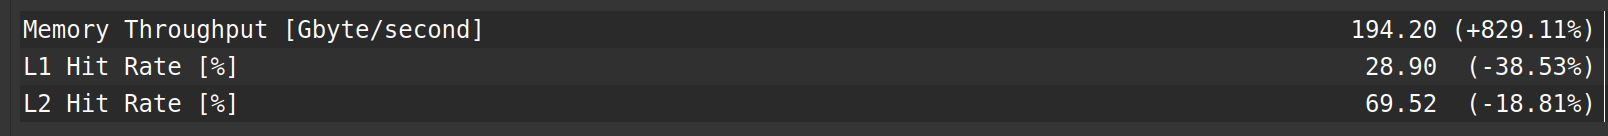
\includegraphics[width=\linewidth]{final_layer2_mem}
        \caption{Memory Throughput}
    \end{subfigure}
    \begin{subfigure}[b]{\linewidth}
        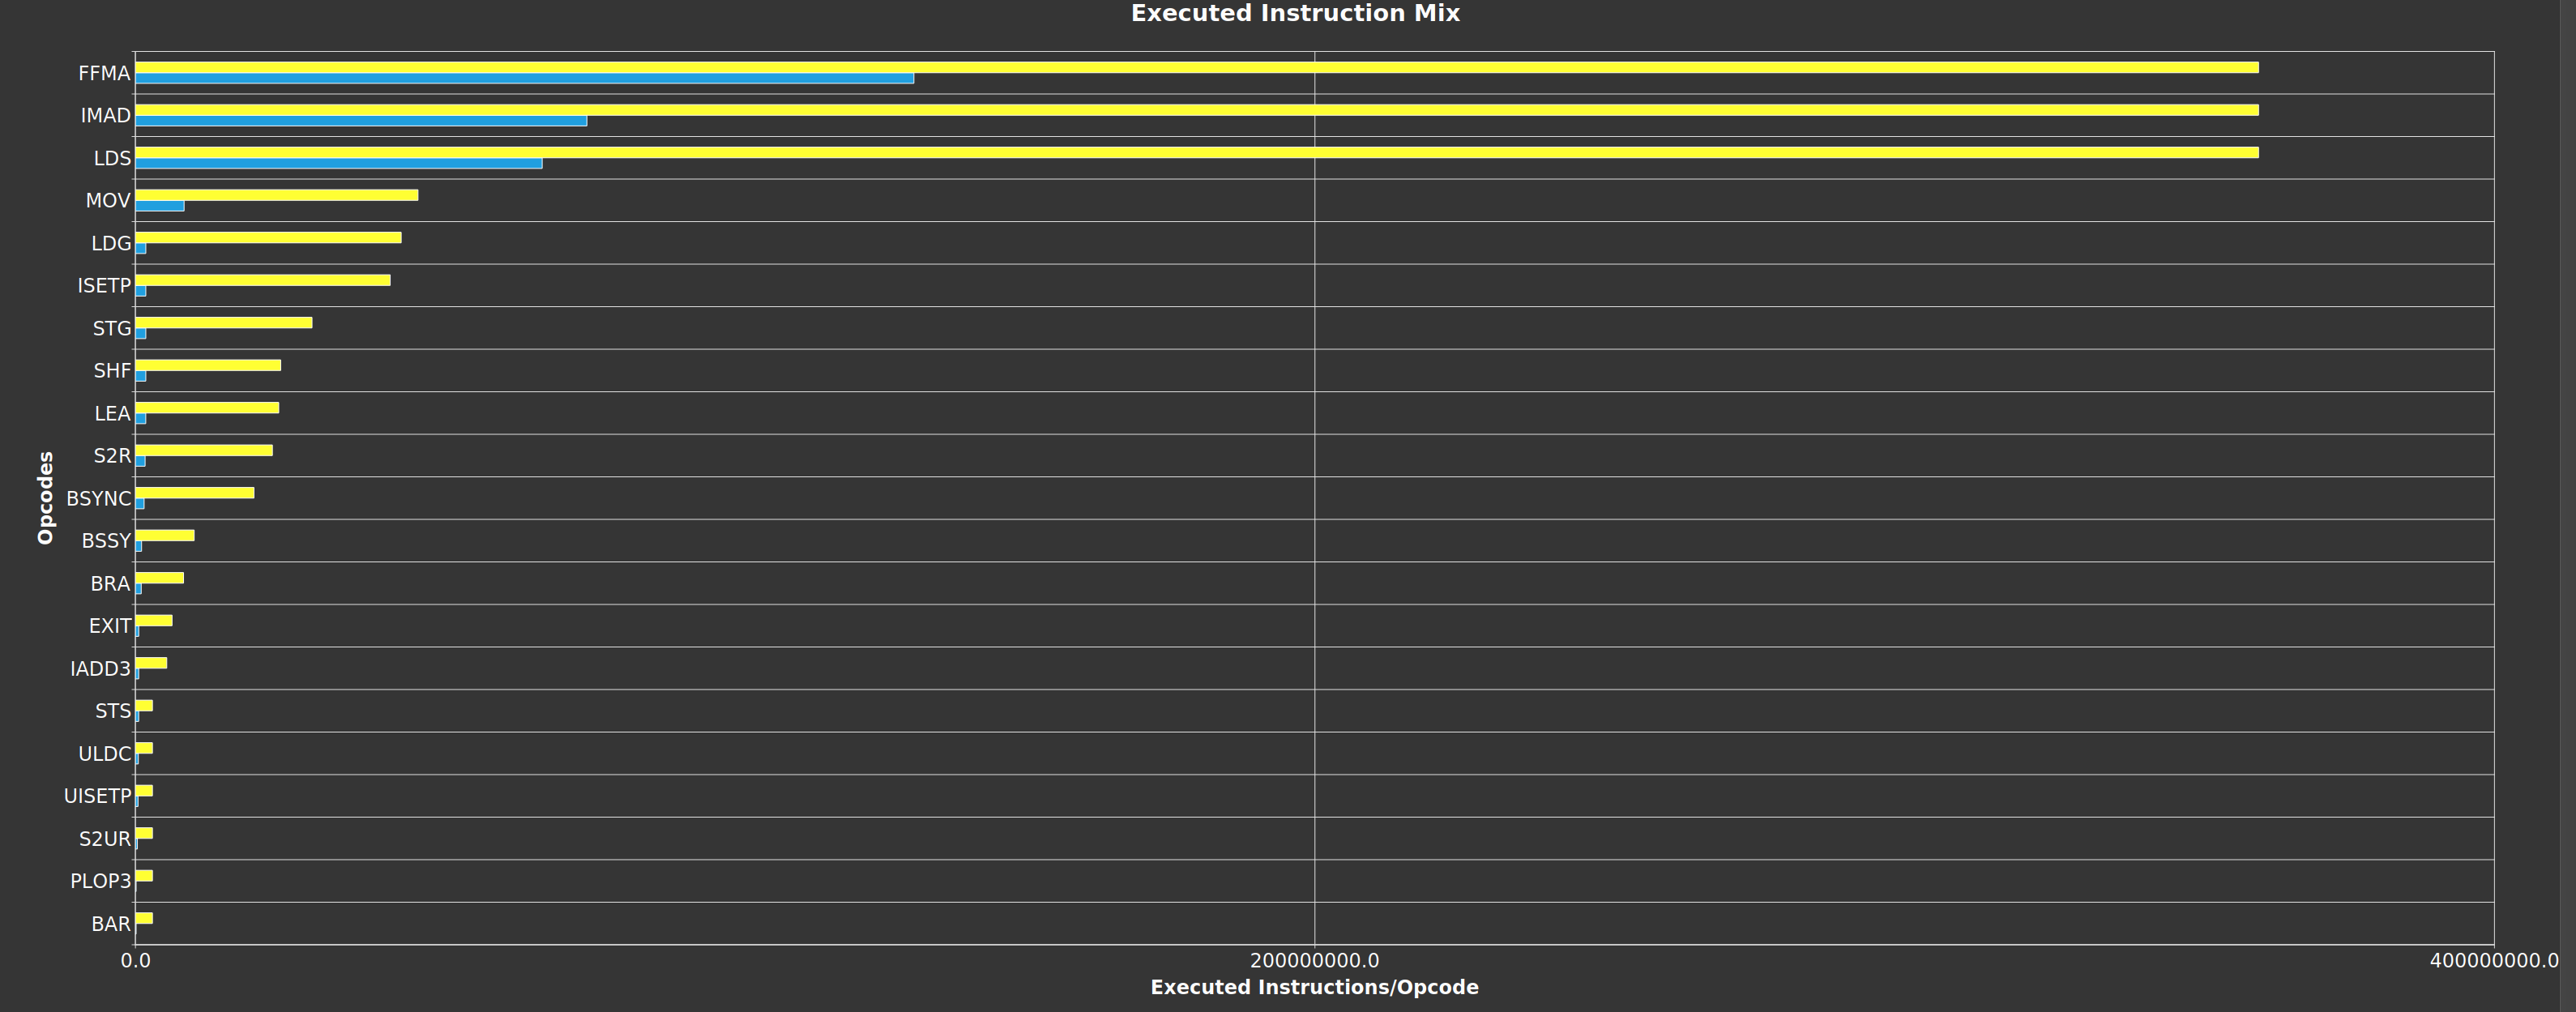
\includegraphics[width=\linewidth]{final_layer2_opcode}
        \caption{Stall Reasons}
    \end{subfigure}
    \caption{Layer 2 Statistics}
\end{figure}

\subsection{More Possibilities}
We acknowledged that there exist many more possibilities of optimization, which we
will only briefly mention here. \\

One possibility is to use FFT (Fast Fourier
Transform) to reduce the Big-O complexity of convolution from $O(n^2)$ to $O(n\text{log}(n))$.
This involves a step to calculate the DFT (Discrete Fourier Transform) of the
convlution kernels and the input feature maps, a step to multiply their DFTs,
and a step to retrieve the final result from the multiplied DFT. While this approach
could theoratically bring a super significant increase in performance, we found it
difficult to adopt in our project because doing FFT introduces too much overheads
that we cannot avoid - for example, zero-padding of input signals is usually done
on the host side, while we already have everything in the device memory. \\

Another possibility is matrix unrolling, which we discussed in class. We actually
implemented a version that uses matrix unrolling as an optimization. However, we did
not see significant performance improvement due to this optimization. We examined
the profling report by Nvidia Nsight Compute and concluded that we have already
achieved a very high memory access efficiency, and thus matrix unrolling does not
help further improve memory access efficiency. However, we did find potential
benefits to implement convolution as matrix multiplication. Since our CUDA device
provides Tensor Cores, which can do matrix multiplication and accumulation with very
high throughput, it is possible to utilize this hardware to do convolution.

\part*{Appendices}
\setcounter{section}{0}

\section{Work Distribution Among Group Members}
Since we are only implementing two kernel functions for the two layers, it is very
hard for us to seperately implement optimizations and combine the work. So for most
of the time, we sat down and do the thinking together, as the majority of time
is spent on the index arithmetic calculations instead of programming itself.
We would like to name this strategy of distributing works "SCMB (Single Computer
Multiple Brains)".

\section{Extra Credit Request}
For each of the optimizations, we performed very thorough analysis to insure we
get the maximum performance gain out of it. The very detailed insights for each and every
optimization are embedded inside the previous analysis sections.\\

The half precision
implementation is especially sophisticated as it involves special caring for both
memory access pattern and compute pattern. Simple change from FP32 to FP16 won't
provide as much of a performance increase as we delivered, especially when our previous
optimization checkpoint already bring us to quite a high performance level, an additional 2x increase
in performance is substantial. Also, the amount of work involved in packing the
data to \verb|half2| pairs and making the new compute logic functional with the new
data structure is at least twice as much as any other optimizations. Hence, we believe that
the additional work put to the last optimization could be potentially considered as
extra credit.\\

Please consider our request.

\end{document}
